\documentclass[a4paper,fleqn]{cas-dc}
\usepackage[numbers]{natbib}

\usepackage{mathtools}
\usepackage{booktabs}

\usepackage{flushend}


\usepackage{graphicx}
\usepackage{algorithm}
\usepackage{algorithmic}
\usepackage{amsmath}
\usepackage{longtable}
\usepackage{array}
\newcolumntype{L}[1]{>{\raggedright\arraybackslash}p{#1}}
\usepackage{amssymb}  % Add this for \mathbb
\usepackage{tikz}
\usepackage{subcaption}
\usepackage{float}
\usepackage{caption}
\usepackage[hypcap=false]{caption}
\usepackage{pgfplots}
\usepackage{standalone}
\pgfplotsset{compat=1.17}

\numberwithin{equation}{section}

\begin{document}
\let\WriteBookmarks\relax
\def\floatpagepagefraction{1}
\def\textpagefraction{.001}

\shorttitle{Scalable Cross-Layer Protocols for Ultra-Dense 
Sensor Network Deployments}
\shortauthors{S Gopikrishnan et~al.}

\title [mode = title]{Scalable Cross-Layer Protocols for Ultra-Dense 
Sensor Network Deployments}                      

%name: Thrishna Katamaneni
%reg no: 23MIS7074
%gmail: thrishnakatamaneni@gmail.com 
%vit-ap mail: thrishna.23mis7074@vitapstudent.ac.in
%orcid: 0009-0006-3145-4373

\author[1]{Thrishna Katamaneni}[orcid=0009-0006-3145-4373]
\ead{thrishna.23mis7074@vitapstudent.ac.in}
\address[1]{School of Computer Science and Engineering, VIT-AP University, Amaravathi. Andhra Pradesh, India}


\cortext[cor1]{Corresponding author}

\begin{abstract}
Ultra-dense sensor networks are being used in a growing number of applications such as smart cities, industrial automation, and environmental monitoring. In such networks, a large number of sensor nodes operate in close proximity, posing challenges in terms of energy consumption, interference, scalability, reliability, and quality of service. These challenges become even more important in ultra-dense networks. The conventional way of organizing network protocols into layers is not suitable for ultra-dense sensor networks as each layer takes decisions based on its local view of the network, without considering other layers. This can lead to inefficient use of resources and reduced network lifetime. Cross-layer protocol design has emerged as a promising way to address these challenges. However, existing solutions either focus on a subset of performance metrics, are not scalable, or assume centralized control which might not be feasible in ultra-dense networks. In this work, we present a distributed cross-layer framework that addresses the energy efficiency, communication reliability, and quality of service concerns in ultra-dense sensor networks by allowing different protocol layers to cooperate closely. To balance the often-conflicting requirements for energy efficiency, reliability, and QoS, we employ multi-objective optimization. The distributed nature of the proposed framework ensures low overhead and good scalability. Through extensive simulations under varying node densities and traffic loads, we compare our framework with a conventional layered protocol approach in terms of network lifetime, packet delivery ratio, latency, and throughput. Our results demonstrate improved performance that makes the proposed framework an attractive choice for next-generation ultra-dense sensing applications.
\end{abstract}

\begin{keywords}
Cross-layer protocols \sep 
Ultra-dense networks \sep 
Wireless sensor networks \sep 
Energy efficiency \sep
Quality of service(Qos) \sep 
 Multi-objective optimization \sep
Scalable architectures \sep
Network Scalability
\end{keywords}

\maketitle

\section{Introduction}

There is an increasing need for Wireless Sensor Networks (WSNs) in various applications such as smart cities, industrial monitoring, environmental sensing and healthcare. This has resulted in the deployment of large scale WSNs with thousands of nodes in small regions – a scenario referred to as ultra-dense WSNs. Although high node densities improve the accuracy of sensing coverage, they also exacerbate some problems associated with WSNs: energy consumption, interference, scalability and quality of service (QoS). Recent surveys have shown that existing protocols do not function efficiently under ultra-dense circumstances and therefore the development of new protocols that take into consideration the challenges associated with density is necessary \cite{Thakur2025}.

Most existing wireless sensor network protocols are based on a strict layered architecture where each layer operates independently from the others. Although this approach makes the protocols easier to design and implement, it results in inefficient resource utilization in dense wireless sensor networks. Studies show that without cross-layer coordination, the protocols experience high energy consumption, increased packet delay, and reduced network lifetime \cite{Amirova2025}. With the increasing demand for ultra-dense wireless sensor network deployments, the need for novel protocols capable of jointly optimizing network lifetime, scalability and reliability becomes more and more urgent \cite{Petrescu2025}.

\subsection{Background and Context}

In an ultra-dense wireless sensor network, there are hundreds to thousands of sensor nodes working at the same time in a small region. In such a network, the main challenges for communication among the nodes are the interferences among them and channel contention, which cause frequent packet collisions and therefore degrade network performance. This situation becomes worse when the density of the nodes increases. As traditional routing and medium access control protocols were initially designed for sparse or moderately dense wireless sensor networks, in an ultra-dense wireless sensor network, they fail to provide the desired performance, which results in increased energy expenditure as well as decreased quality of service \cite{Khamzaev2025498}.

Traditional wireless sensor network protocols are designed based on a layered architecture. Each layer in this architecture is designed to work independently, which makes the protocol design simple but in reality it causes non-optimal performance particularly in densely deployed sensor networks. For instance, routing, transmission power, and other parameters are decided without any coordination among various layers. Such type of protocol design does not provide desired performance when these protocols are employed in high-density wireless sensor networks, resulting in increased latency, increased energy consumption, and packet loss \cite{Cherappa2023}.

Due to limitations such as interference among the nodes and battery life, recent research work has shifted towards cross-layer design. Using this approach information from physical layer, MAC layer and network layer is shared and joint decision is made regarding transmission power, scheduling and routing of data. Since in a dense wireless sensor network we expect more interference, less energy and less quality of service, cross-layer design could be a good solution for dealing with such problems \cite{He2025157}. However cross-layer design that uses centralized approach has scalability problem and hence distributed cross-layer design is used in ultra-dense wireless sensor networks \cite{Mustafa2024}.

\subsection{Research Objectives}

The main objective of this thesis is to design an energy-efficient and scalable cross-layer protocol framework for ultra-dense wireless sensor network deployments. Ultra-dense wireless sensor networks suffer from increased energy consumption due to interference, retransmissions, and inefficiency in protocol layers. The proposed framework will be designed to reduce unnecessary energy consumption by jointly optimizing physical, MAC and network layers while ensuring reliable data transmission. In the ultra-dense wireless sensor network scenario, we need to investigate how cross-layer protocol design can help to save energy without compromising network performance \cite{Singh2025}.

The second objective of the thesis is to develop a distributed cross-layer protocol architecture that can efficiently scale with an increasing number of sensor nodes. Centralized approaches require complete knowledge of the network at the point of decision making resulting in increased overhead due to signaling, reduced adaptability and poor scalability in ultra-dense scenarios. This work is directed towards developing a protocol framework that enables wireless sensor nodes to make autonomous decisions based on their local knowledge. The distributed approach should minimize communication overhead, enhance adaptability and support thousands of wireless sensor nodes in dense deployments \cite{Khamzaev2025498}.

The third objective is to introduce the multi-objective optimization technique to satisfy the conflicting requirements related to energy efficiency, throughput and quality of service. This is necessary because the ultra-dense sensor network has to support multiple applications with different performance requirements. Therefore single objective optimization approach may not be suitable. By framing the optimization problem as multi-objective optimization problem, this work aims at achieving a well balanced trade-off among the important parameters. In addition to that, this work also focuses on adapting to the dynamics of the network such as interference and traffic variations \cite{He2025157}.

The final objective of this paper is to evaluate the efficiency of the cross-layer framework by comparing it with conventional layered protocols using detailed simulations. Simulations are useful in analyzing the behavior of wireless sensor networks such as scalability, energy efficiency, and quality of service performance of the proposed design under various network densities and traffic loads. Performance metrics such as network lifetime, packet delivery ratio, end-to-end delay, and throughput will be used in evaluating and comparing the performance of the proposed framework with traditional layered protocols \cite{Xu2023}.

\section{Literature Survey}

\subsection{Cross-Layer Protocol Design}

This paper proposes a secure and energy-efficient cross-layer network architecture for Internet of Things environments by coordinating operations across multiple protocol layers \cite{Mustafa2025}. In the proposed work, physical layer, MAC layer and network layer are integrated to improve the performance of the network. The main advantage of this cross layer design is that it optimizes the energy consumption as well as improves the security of the network. Therefore, when the number of IoT devices increases, the proposed technique provides a good solution to improve the efficiency of the network. However, the cross layer interaction may introduce additional overhead in terms of processing and communication. Therefore, in case of very dense network such as sensor network, this approach may not be suitable.

This paper focuses on exploring the security and energy efficiency issues in IoT networks via machine learning technologies \cite{Mustafa2O25}. Specifically, we concentrate on discussing the cross-layer design and the learning-based approaches to utilize the cross-layer information for improving the security and energy efficiency. Since machine learning technologies are able to adapt to the changing network environments and make accurate decisions, they have been regarded as a potential solution for tackling various problems in IoT networks. Nonetheless, machine learning technologies also have their own disadvantages. For example, they require intensive computational resources and a large amount of training data. In this sense, when applying machine learning technologies to ultra-dense sensing environments such as those found in certain IoT applications, the implementation of the machine learning models could be challenging.

The proposed framework studies the energy consumption as well as network lifetime by considering the parameters of various protocol layers \cite{Ojeda2024}. Due to consideration of various protocol layers, this work exposes how much energy is wasted at a sensor node because of inefficient coordination among various protocol layers. An important contribution of this work is its detailed energy consumption model for wireless sensor network. However, this work lacks in protocol implementation perspective, since this is an analytical work. In addition, the issue of ultra-dense scenario is not taken into consideration in terms of both scalability and adaptation.

In this paper, a cross-layer routing strategy for opportunistic IoT networks is proposed \cite{Khalil2024}. This strategy leverages information from both physical (PHY) and medium access control (MAC) layers. PHY layer information about link quality and channel condition is exploited at MAC layer for intelligent routing decisions. The proposed strategy adapts dynamically to changing link quality and channel conditions – thus improving both packet delivery ratio and overall network connectivity. The proposed strategy does not depend on fixed paths like traditional routing protocols. However, because continuous cross-layer information exchange between PHY and MAC layers increases signaling overhead, the proposed strategy may be less efficient in very dense IoT networks consisting of a large number of sensor nodes.

A protocol that combines MAC layer scheduling with network layer routing is presented in this paper \cite{Kaddi20242611}. By coordinating these two layers we can reduce idle listening, packet collisions and retransmissions which in turn reduces the energy consumption of the nodes. This cross layer approach results in lower end to end delay with significant improvement in energy efficiency but at the cost of increased complexity. The main disadvantage of such protocols is that they require additional memory and processing power which might not be available on simple sensor nodes. This limits the applicability of such protocol in ultra dense sensor networks.

\subsection{Energy-Efficient Routing Mechanisms}

This work proposes a routing protocol for wireless sensor networks that combines the fuzzy logic, clustering and quantum annealing \cite{Wang2024}. The proposed protocol is designed such that it will select the cluster head intelligently which helps in balancing the energy consumption of the sensor nodes. It increases the network lifetime as well as improves the stability of the network. Although the proposed protocol improves the energy efficiency as well as the stability of the wireless sensor network, still it suffers from certain limitations. The main drawback of the proposed protocol is that it is computationally expensive. Due to this, it may not be feasible to implement the proposed protocol on sensor nodes having limited resources. Secondly, the proposed protocol has not been tested for large-scale and ultra-dense wireless sensor networks consisting of thousands of nodes. It will be interesting to see the performance of proposed protocol in such scenarios.

This paper proposes an energy-efficient routing protocol that combines opportunistic routing and sparse autoencoder \cite{Raj2024122}. The main idea is to compress data via sparse autoencoder before transmitting it to reduce the communication overhead and thus save energy. The advantage of this approach is that it considers both the routing and transmission simultaneously. However, the main disadvantage of this method is that neural networks require training and additional computational resources. Hence, they cannot adapt quickly to changes in real-time scenarios. Moreover, when applied to highly dense and dynamic sensor networks, this approach may not scale well.

This paper proposes a multipath routing algorithm that aims at achieving a good tradeoff between energy efficiency and data accuracy in wireless sensor networks \cite{Dan2024}. The basic idea is to maintain multiple routing paths and adaptively select the forwarding path according to the application-specific accuracy requirement. Such method can improve the fault tolerance ability of data transmission while reducing the unnecessary energy consumption. However, this approach also has some disadvantages, e. g., increasing routing overhead and control message exchange. Moreover, although this method is effective in moderate-density wireless sensor networks, it is still unclear whether this approach can work well in ultra-dense wireless sensor networks.

The use of reinforcement learning in routing protocol design has been investigated in this paper for improving the energy efficiency of software defined networking \cite{Godfrey2023}. It makes use of the characteristics of SDN such as central control and adaptability to decide the optimal routing path dynamically according to the network status. But for dense sensor networks, there exists some disadvantages. For example, the central controller will increase the overhead of control and processing. And all devices depend on central controller. Once the central controller fails, all devices will fail.

Energy-efficient routing protocol for forest fire detection was developed \cite{Pedditi2023}. These protocols are application-specific and incorporate various efficient methods such as priority-based scheduling along with clustering to achieve timely reporting of critical events while reducing the energy expenditure of sensor nodes. Application-specific protocols work well for specific applications but fail to provide a general solution and may not work efficiently in extremely dense environments, as the protocol does not support scalability. They also have limited adaptability in terms of changing environmental conditions.

Routing protocol for wireless sensor networks employing IoT and Dingo is presented in this paper \cite{KishoreKumar2023}. The main aim is to enhance the energy efficiency using optimal routing path. The Dingo algorithm is a nature-inspired optimization algorithm. The main advantage of using this algorithm is that it increases the stability of the network by evenly distributing the energy consumption throughout the network. This increases the lifetime of the network. Also, it has a fast convergence rate compared to other optimization algorithms. But, it increases the computational overhead which is a major disadvantage of all the metaheuristic algorithms. Hence, it is not advisable to use this algorithm for real-time applications. Also, the performance of the algorithm has been tested for small-scale networks. If the network size is very large (i. e. ultra-dense network), the performance of the algorithm degrades.

\subsection{Security and Intrusion Detection}

The proposed framework presents the application of federated learning in detecting cyber threats to IoT-based smart city applications while ensuring data privacy \cite{Ragab2025}. Instead of transmitting raw data, each edge device will train its own model which exchanges model update during global model updating. Data privacy is preserved as raw data isn't transmitted. Security is enhanced with this federated learning approach without exposing the sensitive data of each device, which is critical in IoT applications that consist of a large number of devices. However, there are some challenges with this federated learning-based approach. As it requires continuous exchange of information between the edge devices and central server, the communication overhead increases significantly which may not be suitable for resource-constrained ultra-dense IoT networks consisting of large number of sensing devices. Furthermore, federated learning requires the edge devices to have certain amount of computing resources which might not be always true for all edge devices in an ultra-dense IoT network.

This paper presents a systematic review of intrusion detection methods for IoT networks \cite{Arnob202573}. It highlights the main challenges and future research directions in this area. The intrusion detection methods are categorized based on signature-based, anomaly-based, and hybrid approaches. This paper provides a comprehensive overview of existing solutions. The advantages of this work lie in its thorough analysis of the strengths and weaknesses of different detection methods. However, this paper does not propose any practical intrusion detection framework for IoT networks. Furthermore, most of the surveyed intrusion detection techniques have not been tested in an ultra-dense sensor network environment, which is a typical scenario in many IoT applications.

This paper presents a novel security solution for enhancing the performance of Host-Based Intrusion Detection Systems in IoT networks \cite{Nallakaruppan202431788}. The proposed solution improves the accuracy of detecting intrusion by constantly monitoring system calls from IoT devices, allowing it to detect any suspicious behavior. Although HBIDS are highly efficient at detecting and preventing intrusions while reducing false positives, they do have a major drawback – continuous system monitoring results in heavy energy consumption, making HBIDS less desirable for certain IoT applications where energy resources are limited, such as in dense sensor networks.

This paper presents a machine learning-based intrusion detection system \cite{Almotairi2024}. The proposed system uses feature selection and ensemble learning to improve detection accuracy. Each base classifier is trained on a distinct subset of features. Experimental results show that the proposed system provides high detection accuracy and robustness in detecting various types of attacks. Nonetheless, this method has some drawbacks. It is computationally expensive, and the training dataset size is large. Hence, running this approach on resource-constrained IoT devices with limited processing and memory capabilities is not feasible. Moreover, the issue of scalability in dense sensor networks is not taken into consideration.

This work proposes a security approach based on proxy re-encryption for wireless sensor networks \cite{Khashan202423290}. Data confidentiality is guaranteed through the encryption at source node, and it is protected during transmission via multiple nodes until it reaches destination node, by decrypting and re-encrypting at intermediate sensor nodes. The advantages of this method include strong confidentiality with minimum overhead of key distribution. However, the major disadvantage of this method is that involves complex cryptographic computations that increase the energy expenditure of nodes and reduce the network lifetime as well as the scalability of WSN.

\subsection{Quality of Service and Dense Network Optimization}

This paper proposes a novel optimization approach to improve the quality of service in a heterogeneous IoT sensor network \cite{Vatankhah2024}. The proposed method utilizes the multi-objective scheduling algorithm for time-slotted channel hopping to optimize the key performance indicators such as latency, reliability, and energy efficiency. One major benefit of using the proposed multi-objective optimization approach is that it can manage different conflicting requirements. Hence, the proposed approach can be used to maintain the QoS in dense IoT sensor networks where a variety of applications are supported. However, the major drawback is that the computational complexity associated with the proposed approach is high and requires precise information about the network state to achieve the optimal results. Therefore, to achieve real-time optimization, the proposed approach is required to be adapted to handle the highly dynamic traffic in ultra-dense IoT sensor networks.

In order to improve the scalability and reliability of linear wireless sensor networks in smart cities, this paper proposes a queuing strategy \cite{Villordo-Jimenez2024}. Packets are given priority based on their distance from the receiving node and current network conditions. This reduces congestion and loss of packets caused by collisions. The advantage of this strategy is increased throughput and reduced delay in heavy traffic. However, it is most suitable for networks with a linear structure. In complex or irregular network topologies, its performance may not be optimal. Furthermore, this strategy may not adapt well to ultra-dense wireless sensor networks that change very frequently.

This paper proposes an optimization framework for 5G in IoT applications \cite{Pons2023}. This work focuses on interference management and optimization problems in IoT networks enhanced with 5G. The introduction of 5G in IoT applications is important in increasing the data rates and reducing the latency of IoT networks; especially dense IoT networks. The framework is able to identify key limiting issues in IoT networks such as interference and resource allocation problems. However, 5G based solutions may not be suitable for all types of IoT applications; especially low power consumption ultra dense sensing applications due to the expensive nature of 5G infrastructures and devices.

An innovative system-level integration solution is presented in this paper \cite{Ficili2025}. The Internet of Things (IoT), cloud computing, edge computing and artificial intelligence are combined in order to improve data processing and decision-making. Computation is performed across both edge and cloud layers in the proposed framework. The distribution of computation in this way reduces the latency and improves the quality of service in large-scale deployments compared to traditional cloud-based approaches. System-level integration of edge, IoT and AI offers the potential for improved scalability and better support for data-intensive applications. However, this approach relies heavily on reliable connectivity as well as sufficient infrastructure support, limiting its potential when it comes to simple, resource-constrained devices deployed in ultra-dense networks.

\subsection{Research Gaps}

The first research gap identified is the absence of a common cross-layer framework that can jointly optimize the most important performance metrics of ultra-dense sensor networks. Indeed, most of today’s cross-layer solutions have been designed with a single goal in mind, be it to reduce energy consumption, latency or boost throughput. While this may bring benefits in certain situations, these approaches do not take into account the trade-offs that exist between different performance requirements. Hence, what is needed is a cross-layer framework that can balance energy, QoS and scalability.

The second gap relates to how well cross-layer protocols scale when they are running on a distributed system. A lot of the research in this area has been based on centralised control or needing information about the whole network. This can create problems as the number of devices (nodes) increases because there is more signalling traffic and it becomes harder to process information in real-time. Even when distributed solutions are proposed they often assume the network will not change much or that there will not be many nodes. This means there is a need for fully distributed, cross-layer protocols that can work well even when the network is very dense and changing a lot – like you would expect in a swarm of sensors. Such protocols should also be lightweight.

The third research gap relates to the integration of security and reliability in cross-layer design for wireless sensor networks. In general, a base paper may focus on energy and/or throughput optimization but may well consider reliability and security as an add-on extra – often resulting in cross-layer solutions that don’t perform well in a real-world wireless sensor network environment where attacks, link errors, and tampering are a norm. Therefore, there exists a need to develop a cross-layer protocol design solution which can simultaneously optimize for energy efficiency, reliability, and security without sacrificing too much overhead.

The fourth gap relates to performance evaluation in realistic ultra-dense network conditions. Specifically, existing studies typically evaluate their cross-layer solution proposals using simplistic simulators and scenario setups, such as limited numbers of nodes, stationary traffic load and so on. As a result, it remains unclear if and how these solutions operate effectively when deployed in ultra-dense networks where interference and collision levels are typically very high and traffic is dynamic. Therefore comprehensive simulation evaluations of cross-layer solutions that take into account different network densities and a range of performance metrics are necessary in order to determine which solutions work well in practice.

\subsection{Motivation}

There is an increasing need for ultra-dense sensor networks in various applications including but not limited to smart cities, industrial sensing as well as environmental monitoring. However, with the increased demand, there are challenges associated with ultra-dense sensor networks which include but are not limited to energy consumption, interference, scalability as well as communication reliability. In traditional layered protocols, each layer is independent and thus, when decisions are taken at a particular layer, the impact on other layers is not taken into consideration. Such an approach leads to inefficient usage of resources resulting in reduced network lifetime and this calls for new approaches to overcome the challenges associated with ultra-dense sensor networks.

Cross-layer protocol design can address the challenges mentioned above by enabling information sharing and collaborative decision making between different protocol layers. Joint optimization of transmission power, routing and scheduling can significantly improve network performance. Current cross-layer protocols for sensor networks have several limitations including poor scalability and adaptability. The complexity of cross-layer protocols, as well as simplifying assumptions that do not hold in ultra-dense and dynamic sensor networks, hinders the application of these protocols in real-world environments.

Motivated by the above difficulties in existing sensor network protocols and the need for next-generation applications, we focus on designing a cross-layer framework that is distributed and scalable, and suitable for ultra-dense sensor networks. We aim at developing a protocol stack that provides a good trade-off between energy efficiency, reliability, Quality of Service (QoS), and overhead. The framework is designed such that it overcomes the limitations discussed above, and is simple to implement in real-world applications. This way, we can enhance the overall performance of the sensor network.

\subsection{Problem Statement}

The main issue with existing solutions is that they were developed using the traditional protocol stack approach. Specifically, current solutions minimize energy consumption at each layer independently. It has been shown that independent optimization of protocol layers does not lead to global optimization of network energy consumption. As a result, in an ultra-dense environment, the overall energy consumption of the network is very high and the network lifetime is very low. In the context of sensor networks, this work is dedicated to proposing a cross-layer framework to minimize energy consumption while maximizing network reliability. In other words, this research aims at investigating the design space of a cross-layer framework that takes advantage of inter-layer synergies to achieve energy efficiency.

Another critical issue with cross-layer approaches is their limited scalability, which becomes particularly important when dealing with large-scale wireless sensor networks. A lot of existing solutions rely on central control or need information about the whole network. These requirements can lead to a large amount of signaling traffic and reduced adaptability. As the network scales up and topology changes become more frequent— as is the case in ultra-dense wireless sensor networks— this may not be practical. Interference is another issue that could affect performance in such scenarios. In this project we aim at investigating distributed cross-layer solutions that can scale well and make use of only local information.

Another issue is that majority of the current protocols are designed with a single objective in mind and therefore fail to strike the right balance between important performance parameters like energy efficiency, throughput, latency and quality of service (QoS). This means that when one parameter is optimised it has a negative impact on another. With ultra-dense wireless sensor networks in mind, it is necessary to develop new cross-layer strategies which take multiple objectives into consideration at once; these protocols should also be able to adapt as network conditions change if they are going to meet the challenges posed by future applications.

Finally, most existing cross-layer protocols are tested in simulation environments that do not accurately reflect real-world ultra-dense network conditions. As a result, their performance in such networks cannot be reliably predicted from simulations. Network simulations that only consider simple scenarios with low numbers of nodes and static data traffic patterns cannot provide a realistic basis for evaluating cross-layer protocols, especially in ultra-dense networks where things are much more complicated. Moreover, the performance metrics considered in simulations are usually limited, for example, delay and throughput. The proposed cross-layer protocol is evaluated through simulation. However, unlike most studies that consider simple scenarios, we simulate various network densities to better understand how well our protocol works under different conditions. We also consider multiple performance metrics to get a more complete picture of its advantages and disadvantages.

\begin{table*}[htbp]
\centering
\caption{Literature Survey Summary}
\label{tab:literature_summary}
\footnotesize
\renewcommand{\arraystretch}{1.2}
\setlength{\extrarowheight}{2pt}
\begin{tabular}{|L{0.85cm}|L{3.4cm}|L{3.0cm}|L{3.2cm}|L{3.7cm}|}
\hline
\textbf{Ref.} & \textbf{Method Proposed} & \textbf{Techniques Used} & \textbf{Issues Resolved} & \textbf{Limitations} \\
\hline

\cite{Thakur2025} & Comprehensive review of AI-driven energy-efficient routing approaches for IoT-based wireless sensor networks & Machine learning models, artificial intelligence techniques, routing optimization, energy-aware decision mechanisms & Identification of energy-efficient routing strategies, analysis of strengths and weaknesses, and highlighting open research challenges & Review-oriented study without experimental validation, limited discussion on real-time implementation and ultra-dense network scalability \\
\hline

\cite{Asaithambi2025} & Blockchain-assisted edge computing architecture designed for secure and trustworthy Industrial IoT systems & Blockchain technology, edge computing, smart contracts, distributed consensus mechanisms & Improved data integrity, decentralized authentication, and trust management in industrial IoT environments & High computational and storage overhead of blockchain, limited suitability for resource-constrained sensor nodes and dense deployments \\
\hline

\cite{Petrescu2025} & Comprehensive survey of transport and application layer communication protocols for Internet of Things & Protocol analysis, layered communication models, performance benchmarking, reliability comparison & Clear classification of IoT protocols and guidance for protocol selection based on application requirements & Survey-based analysis lacking implementation results, minimal focus on cross-layer interaction and energy efficiency aspects \\
\hline

\cite{Kim2022} & Cross-layer MAC and routing protocol aimed at improving communication reliability in IoT networks & MAC-routing coordination, packet scheduling strategies, reliability-aware protocol design & Enhanced packet delivery reliability and reduced packet loss through coordinated layer interaction & Based on older network assumptions, limited scalability analysis, not evaluated under ultra-dense sensor network conditions \\
\hline

\cite{Firdous2022} & Cluster-based routing approach for efficient energy management in IoT-assisted wireless sensor networks & Clustering techniques, hierarchical routing, energy-aware communication mechanisms & Balanced energy consumption among nodes and prolonged overall network lifetime & Static clustering structure, limited adaptability to dynamic traffic, reduced effectiveness in highly dense environments \\
\hline

\cite{Nguyen2022} & Lightweight network intrusion detection system deployed at IoT gateway level & Traffic monitoring, anomaly detection techniques, lightweight IDS architecture & Early detection of network-level attacks with low computational overhead at gateways & Gateway-centric design unable to detect node-level attacks, scalability limitations in large-scale networks \\
\hline

\cite{Kamaldeep202128066} & Cross-layer intrusion detection system utilizing information from multiple protocol layers in IoT & Cross-layer feature extraction, protocol-aware intrusion detection, anomaly-based analysis & Improved detection accuracy by correlating features across protocol layers & High feature extraction complexity, increased processing overhead, limited suitability for ultra-dense sensor networks \\
\hline

\cite{Diamantoulakis2021} & Optimization framework for performance enhancement in ultra-dense wireless powered networks & Wireless power transfer, energy harvesting models, network optimization techniques & Improved energy utilization and performance in dense wireless powered communication environments & Strong theoretical focus, limited practical validation for real-world sensor network deployments \\
\hline

\cite{Cerar2020212130} & Machine learning-based framework for detecting anomalous wireless links in IoT networks & Supervised learning, anomaly detection models, wireless link performance analysis & Accurate identification of abnormal link behavior that degrades network performance & Dependence on labeled training data, limited evaluation in large-scale and ultra-dense network scenarios \\
\hline

\cite{Ruiz2011} & Cross-layer medium access control protocol with quality-of-service guarantees for wireless sensor networks & MAC scheduling, QoS-aware design, cross-layer coordination mechanisms & Guaranteed delay and throughput for priority traffic flows & Older protocol design, limited adaptability to modern dynamic and ultra-dense sensor networks \\
\hline

\cite{Alsharif202311197} & Intrusion detection framework combining machine learning and blockchain for IoT security & Machine learning-based attack detection, blockchain-based data integrity, security analytics & Enhanced intrusion detection accuracy and secure data management in IoT systems & Increased system complexity and overhead, not suitable for low-power or ultra-dense sensor deployments \\
\hline

\end{tabular}
\end{table*}

\section{Proposed Work}

Ultra-dense sensor network deployments requires efficient communication technologies to deal with a large number of sensor nodes in a limited geographical area. Traditional layered protocol stacks suffer from poor layer coordination, leading to high energy consumption, communication delays and packet losses in dense network conditions. To address the challenges in these networks, a scalable cross-layer routing framework called the Scalable Cross Layer Routing Protocol (SCLRP) is proposed. The proposed SCLRP framework enhances communication efficiency by enabling information sharing among protocol layers. It integrates network layer routing decisions, MAC layer scheduling information and physical layer link quality indicators to improve overall network performance.

The main objective of the proposed SCLRP framework is to improve energy efficiency, reliability and scalability in ultra-dense sensor network deployments. The proposed SCLRP framework enables cross-layer communication, allowing routing decisions to take into consideration parameters such as remaining node energy, link quality and network congestion level. The coordinated approach to reducing unnecessary packet retransmissions leads to improved packet delivery performance. The proposed SCLRP framework is designed to adapt to varying levels of network density and traffic patterns. The Scalable Cross Layer Routing Protocol framework is described in Fig. \ref{fig_framework}, which outlines how information from multiple layers can be used to make efficient routing and transmission decisions.

\begin{figure*}[t]
\centering
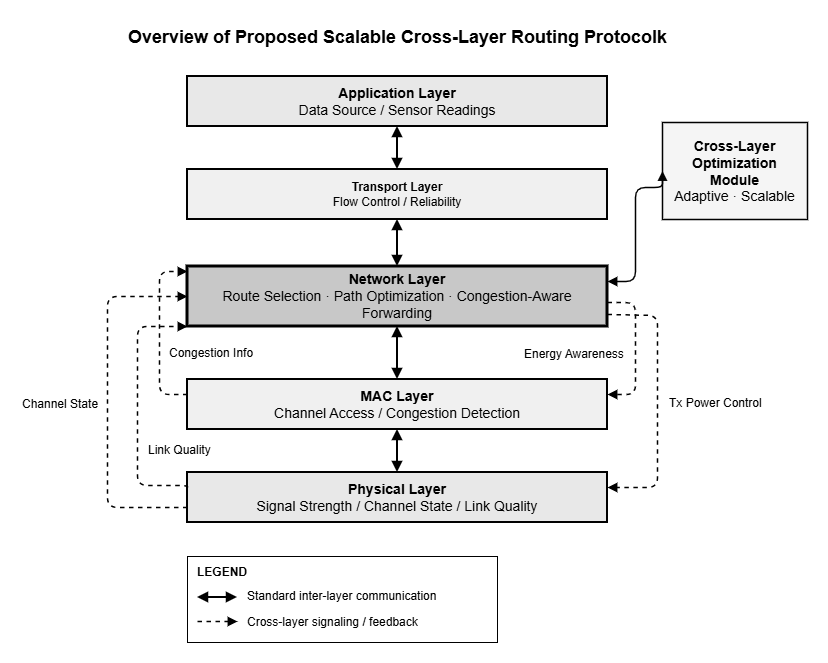
\includegraphics[width=\textwidth]{figures/framework_diagram.png}
\caption{Overview of the Proposed Scalable Cross Layer Routing Framework}
\label{fig_framework}
\end{figure*}

\subsection{Overview of Proposed Framework}

The proposed scalable cross layer framework enables coordinated interaction among multiple communication layers in order to improve network performance in conditions of very high network density. In the conventional layered communication systems, each layer of the protocol stack operates independently and does not make use of the information available at other layers. Such a approach can lead to inefficient use of resources in dense sensor networks where high energy consumption, interference and congestion are major challenges. The proposed framework addresses these challenges through enabling controlled information exchange between the physical layer, medium access control layer and network layer.

The physical layer provides information about the signal strength and link quality that can be used to assess the reliability of communication between neighboring nodes. The medium access control layer provides information about channel usage and local traffic congestion conditions. The network layer based on this information selects the optimal routing paths that reduce energy consumption and provide reliable communication. By combining the information from multiple layers, the proposed framework offers better opportunities to take informed decisions about routing and transmission compared to the traditional layer based protocols.

The architecture of the proposed scalable cross-layer framework is shown in Fig. \ref{fig_framework}. The framework explains how link quality information from the physical layer and channel state information from the medium access control layer are used by the network layer to determine the routing paths. Good link quality information and channel state information contribute to a stable network and minimize communication overhead in ultra-dense deployments. The framework also includes adaptive transmission control capabilities that enable good network performance even as the node density increases. Effective cross-layer communication is necessary to achieve scalable communication in large-scale sensor network environments.

\subsection{System Model}

The proposed scalable cross-layer framework is designed for ultra-dense wireless sensor network deployments where a large number of sensor nodes are deployed in a limited geographical area. The network consists of static sensor nodes that are randomly scattered throughout the sensing region. Each sensor node is equipped with sensing capabilities, wireless communication interfaces, limited processing capabilities, and limited energy resources. All nodes use multi-hop wireless communication to send sensed data to a sink node that collects data from the network. The communication process relies on the cooperative interaction of physical layer, medium access control layer and network layer to enable efficient data transfer.

The sensing area is represented by a square region in which a set of sensor nodes are deployed. The total number of sensor nodes in the network is denoted by N. Each node periodically generates sensing data and forwards it to the sink node using multi-hop routing. The distance between two sensor nodes is important in calculating the transmission energy and communication reliability. The Euclidean distance between node i and node j can be calculated using Eq. \ref{eq_distance_model}. This distance metric is used to calculate the communication cost during the route selection process.

\begin{equation}
d_{ij} = \sqrt{(x_i - x_j)^2 + (y_i - y_j)^2}
\label{eq_distance_model}
\end{equation}

The energy needed to send a packet from node i to node j is based on the communication distance and radio transmission characteristics. The energy required to send a packet is described by Eq. \ref{eq_transmission_energy}. The equation describes the relationship between the transmission distance and the required energy in dense wireless communication networks.

\begin{equation}
E_{tx} = E_{elec} \times L + \epsilon_{amp} \times L \times d_{ij}^2
\label{eq_transmission_energy}
\end{equation}

Energy consumed during packet reception contributes to the total energy used by the sensor node. The energy model for reception is given in Eq. \ref{eq_reception_energy}. The energy model is required to determine the lifetime of the node and ensure the overall sustainability of the network.

\begin{equation}
E_{rx} = E_{elec} \times L
\label{eq_reception_energy}
\end{equation}

The total communication energy of a node is calculated by considering both the transmission and reception energy consumption. The energy consumption model is described by Eq. \ref{eq_total_energy}. The proposed framework uses this equation to monitor the state of node energy during routing and transmission control.

\begin{equation}
E_{total} = E_{tx} + E_{rx}
\label{eq_total_energy}
\end{equation}

The quality of communication links between adjacent nodes is a significant factor in route choice decisions. The quality of a link is estimated based on the received signal strength indicators that describe the communication channel conditions between communicating nodes. The link quality metric is calculated based on Eq. \ref{eq_link_quality}. High link quality values indicate good quality communication links.

\begin{equation}
LQ_{ij} = \frac{P_r}{P_t}
\label{eq_link_quality}
\end{equation}

The network also considers the residual energy of nodes when selecting the forwarding nodes. Residual energy refers to the amount of energy available at each sensor node after it has been used to perform sensing, processing, and communication tasks. The residual energy value is obtained from Eq. \ref{eq_residual_energy}. The residual energy parameter helps to avoid nodes with very low levels of energy during the routing process.

\begin{equation}
RE_i = E_i - E_{consumed}
\label{eq_residual_energy}
\end{equation}

The parameters given in Eqs. \ref{eq_distance_model} to \ref{eq_residual_energy} provide a basic mathematical description of the network model used in the proposed scalable cross-layer framework. These parameters are continuously monitored and shared across communication layers to enable effective routing, energy-aware transmission and congestion management in ultra-dense sensor networks.

\subsection{Phase 1: Node State Evaluation}

The SCLRP framework's first phase is to conduct node state evaluation to enable efficient routing and data transmission strategies in highly dense sensor network environments. Each sensor node is assumed to monitor its operating state to provide the necessary information required to make decisions at the cross-layer level. The state of the node includes the residual energy level, communication link quality, density of neighboring nodes, congestion level and capacity to forward packets. The necessary information is gathered at each node and reported to the Cross Layer Information Manager. The process of evaluating the node state enables the routing decisions to identify reliable and energy efficient nodes that can be used to forward data packets.

The residual energy of a sensor node represents the amount of energy available after the tasks of sensing, processing and communication are performed. Residual energy can be calculated using Eq. \ref{eq_phase1_residual_energy}. High levels of residual energy indicate that a node can participate in routing tasks for a longer period of time.

\begin{equation}
RE_i = E_i - E_{used}
\label{eq_phase1_residual_energy}
\end{equation}

The node energy ratio indicates the proportion of available energy with respect to the initial node energy. The energy ratio is calculated using Eq. \ref{eq_energy_ratio}. The energy ratio allows the routing system to compare nodes with varying levels of remaining energy.

\begin{equation}
ER_i = \frac{RE_i}{E_{init}}
\label{eq_energy_ratio}
\end{equation}

The quality of the link between two nodes is determined using received signal strength measurements. The link quality model is described in Equation \ref{eq_phase1_link_quality}. Good links give higher values of link quality.

\begin{equation}
LQ_{ij} = \frac{P_r}{P_t}
\label{eq_phase1_link_quality}
\end{equation}

The reliability of communication between adjacent nodes is also affected by the packet success probability. The value of this parameter is calculated using Eq. \ref{eq_packet_success}.

\begin{equation}
PS_{ij} = \frac{S_{pkt}}{T_{pkt}}
\label{eq_packet_success}
\end{equation}

The congestion state of a node can be estimated based on the packet queue occupation at the medium access control layer. The congestion index is calculated based on Eq. \ref{eq_congestion_index}.

\begin{equation}
CI_i = \frac{Q_i}{Q_{max}}
\label{eq_congestion_index}
\end{equation}

Neighbor density is a key aspect of ultra dense networks since excessive neighboring devices can lead to increased levels of interference and routing complexities. The neighbor density of a node can be calculated using Eq. \ref{eq_neighbor_density}.

\begin{equation}
ND_i = \sum_{j=1}^{N} A_{ij}
\label{eq_neighbor_density}
\end{equation}

The node reliability score combines information about the node's energy and communication capacity in order to estimate its ability to forward data. The reliability score can be calculated from Eq. \ref{eq_reliability_score}.

\begin{equation}
RS_i = ER_i \times LQ_{ij}
\label{eq_reliability_score}
\end{equation}

The forwarding capability metric reflects a node's ability to act as an intermediate routing node. The value of this parameter can be obtained from Eq. \ref{eq_forwarding_capability}.

\begin{equation}
FC_i = RS_i \times PS_{ij}
\label{eq_forwarding_capability}
\end{equation}

The node state weight represents the combined effect of energy condition, link quality and level of congestion. The node weight is calculated using Eq. \ref{eq_node_weight}.

\begin{equation}
NW_i = \alpha ER_i + \beta LQ_{ij} + \gamma CI_i
\label{eq_node_weight}
\end{equation}

The final node state value defined in the framework is used to guide routing decisions based on the reliability and ability to forward metrics. The evaluation of the final state is described in Eq. \ref{eq_final_state}.

\begin{equation}
NS_i = NW_i + FC_i
\label{eq_final_state}
\end{equation}

The parameters listed in Eq. \ref{eq_phase1_residual_energy} to Eq. \ref{eq_final_state} enable the proposed framework to model the operating state of each node in the network. These parameters are conceptually updated and used within the framework to support cross-layer decision-making (evaluated through simulation).

\begin{algorithm}
\caption{Node State Evaluation}
\begin{algorithmic}[1]
\REQUIRE 
    $T_{interval}$: monitoring time interval;
    $E_{init}$: initial energy value;
    $\alpha, \beta, \gamma$: weight coefficients for state evaluation;
\STATE Initialize sensor node $i$;
\STATE $E_i \leftarrow E_{init}$;
\STATE Start sensing operation and monitor packet generation;
\REPEAT
    \STATE Detect neighboring nodes $j$;
    \STATE Estimate communication distance $d_{ij}$ and measure received signal strength $P_r$;
    \STATE Compute link quality value $LQ_{ij}$ and calculate packet success probability $PS_{ij}$;
    \STATE Monitor queue occupancy and estimate congestion index $CI_i$;
    \STATE Determine neighbor density $ND_i$;
    \IF{$E_i - E_{used} > 0$}
        \STATE Calculate residual node energy $RE_i \leftarrow E_i - E_{used}$;
        \STATE Compute energy ratio $ER_i \leftarrow \frac{RE_i}{E_{init}}$;
        \STATE Evaluate node reliability score $RS_i \leftarrow ER_i \times LQ_{ij}$;
        \STATE Estimate forwarding capability $FC_i \leftarrow RS_i \times PS_{ij}$;
        \STATE Compute node state weight $NW_i \leftarrow \alpha ER_i + \beta LQ_{ij} + \gamma CI_i$;
        \STATE Determine final node state value $NS_i \leftarrow NW_i + FC_i$;
        \STATE Update cross layer information database;
        \STATE Share node state information $NS_i$ with routing engine;
        \STATE Wait for $T_{interval}$;
    \ELSE
        \STATE Node $i$ is depleted of energy;
        \RETURN
    \ENDIF
\UNTIL{sensing operations are terminated}
\end{algorithmic}
\end{algorithm}

\subsection{Phase 2: Cross Layer Routing Decision}

The second part of the proposed SCLRP framework defines a routing decision model based on the information obtained during node state evaluation. Ultra-dense sensor networks have a large number of nodes competing for communication resources. Conventional routing protocols based on hop count lead to network congestion, excessive number of packet retransmissions and uneven energy consumption throughout the network. The proposed cross-layer routing strategy utilizes information from physical layer, medium access control layer and network layer to identify an efficient data forwarding route.

Within the proposed framework, routing decisions are based on node state informatio from the cross layer information manager. This information includes available energy, link quality, traffic congestion level and the ability to forward data. The framework defines a routing decision strategy that identifies a set of candidate nodes and selects the best one to act as the next hop for forwarding the packets. The routing cost metric combines several parameters necessary to determine the performance of the network. The formula for calculating the routing cost is given by Eq. \ref{eq_routing_cost_base}. A lower routing cost indicates a more suitable forwarding node.

\begin{equation}
RC_{ij} = w_1 RE_i + w_2 LQ_{ij} + w_3 CI_i
\label{eq_routing_cost_base}
\end{equation}

The reliability of routing also depends on the probability of successful packet delivery. The packet delivery metric between two nodes is obtained using Eq. \ref{eq_delivery_ratio}. This value reflects the ratio of successfully delivered packets to the total number of transmitted packets.

\begin{equation}
DR_{ij} = \frac{P_{success}}{P_{total}}
\label{eq_delivery_ratio}
\end{equation}

Communication delay between nodes also affects routing decisions. The delay estimation model is described in Eq. \ref{eq_delay_estimation}. The value represents the time required for a packet to be transmitted from node i to node j.

\begin{equation}
D_{ij} = \frac{L}{R}
\label{eq_delay_estimation}
\end{equation}

Improved routing efficiency is obtained when nodes with high energy and reliable links are selected as intermediate forwarding nodes. The routing efficiency metric is expressed as in Eq. \ref{eq_routing_efficiency}.

\begin{equation}
REFF_{ij} = RE_i \times DR_{ij}
\label{eq_routing_efficiency}
\end{equation}

In ultra dense network deployments, node congestion can impact the routing performance. The congestion adjusted routing metric is defined in Eq. \ref{eq_congestion_adjusted}.

\begin{equation}
CA_{ij} = \frac{REFF_{ij}}{CI_i}
\label{eq_congestion_adjusted}
\end{equation}

The routing priority score assesses the candidate neighbors based on their energy level and link reliability. The routing priority metric is given in Eq. \ref{eq_priority_metric}.

\begin{equation}
RP_{ij} = LQ_{ij} + RE_i
\label{eq_priority_metric}
\end{equation}

The neighbor suitability metric evaluates a node's ability to forward packets efficiently. The neighbor suitability metric is defined as described in equation \ref{eq_neighbor_suitability}.

\begin{equation}
NS_{ij} = RP_{ij} \times DR_{ij}
\label{eq_neighbor_suitability}
\end{equation}

The path quality estimation takes into account the cumulative reliability of nodes along the path to the sink node. The path quality index is represented by Eq. \ref{eq_path_quality}.

\begin{equation}
PQ = \sum NS_{ij}
\label{eq_path_quality}
\end{equation}

The routing decision score combines route quality and traffic information to choose the best route. The routing score is given by Eq. \ref{eq_route_score}.

\begin{equation}
RS = \frac{PQ}{CI_i}
\label{eq_route_score}
\end{equation}

The framework suggests selecting the next hop node based on the highest routing score value.. The selection of this criterion is based on equation \ref{eq_next_hop_selection}

\begin{equation}
NH = \max RS
\label{eq_next_hop_selection}
\end{equation}

The equations defined in Eq. \ref{eq_routing_cost_base} through Eq. \ref{eq_next_hop_selection} provide the mathematical basis used by the cross-layer routing decisions defined in the framework. The metrics defined in the proposed framework enable the evaluation of candidate nodes based on energy consumption, link reliability, level of congestion and packet delivery capability. These metrics are conceptually updated within the framework and are evaluated through simulation.

\begin{algorithm}
\caption{Cross Layer Routing Decision}
\begin{algorithmic}[1]
\REQUIRE 
    Neighbor node table; 
    Cross layer information database;
\STATE Receive node state information for candidate nodes;
\REPEAT
    \STATE Access neighbor node table and collect residual energy values;
    \STATE Obtain link quality measurements and monitor congestion level;
    \STATE Estimate packet delivery ratio $DR_{ij} \leftarrow \frac{P_{success}}{P_{total}}$;
    \STATE Evaluate communication delay $D \leftarrow \frac{L}{R}$;
    \STATE Compute routing efficiency $REFF_{ij} \leftarrow RE_i \times DR_{ij}$;
    \STATE Calculate congestion adjusted metric $CA_{ij} \leftarrow \frac{REFF_{ij}}{CI_i}$;
    \STATE Determine routing priority score $RP_{ij} \leftarrow LQ_{ij} + RE_i$;
    \STATE Evaluate neighbor suitability $NS_{ij} \leftarrow RP_{ij} \times DR_{ij}$;
    \STATE Estimate path quality value $PQ \leftarrow \sum NS_{ij}$;
    \STATE Compute routing score $RS \leftarrow \frac{PQ}{CI_i}$;
    \IF{candidate nodes exist}
        \STATE Select node with maximum routing score $NH \leftarrow \max(RS)$;
        \STATE Update routing table and assign selected node as next hop;
        \STATE Forward packet to selected node;
        \STATE Monitor packet transmission result and update routing metrics;
    \ELSE
        \STATE Drop packet or initiate route discovery;
        \RETURN
    \ENDIF
\UNTIL{no more packets to route}
\end{algorithmic}
\end{algorithm}

\subsection{Phase 3: Adaptive Transmission Control}

The third phase of the proposed SCLRP framework defines adaptive transmission control strategies to ensure efficient communication in ultra-dense sensor network environments. The networks are comprised of a large number of sensor nodes that attempt to send data simultaneously, resulting in increased interference, data packet collisions, and energy consumption. The adaptive transmission control mechanism is designed to dynamically adjust the transmission parameters based on the network conditions such as node density, level of congestion and link quality. Based on information obtained from physical layer, medium access control layer and network layer, this phase focuses on managing and improving the network's ability to communicate effectively and enhance overall network performance.

The transmission power needed for communication between two nodes depends on the distance between them and the required signal strength. The transmission power model is described by Eq. \ref{eq_tx_power}. The equation defines how transmission power can be set based on the communication distance.

\begin{equation}
P_t = P_{min} + k \times d_{ij}
\label{eq_tx_power}
\end{equation}

The received signal strength is affected by channel conditions and interference from neighboring nodes. The received signal strength model is formulated by Eq. \ref{eq_rx_power}. This value can be used to estimate the reliability of communication.

\begin{equation}
P_r = \frac{P_t}{d_{ij}^2}
\label{eq_rx_power}
\end{equation}

The signal to interference ratio is a measure of the quality of the communication channel. It is calculated by means of Eq. \ref{eq_sir}. Higher values correspond to better conditions for communication.

\begin{equation}
SIR = \frac{P_r}{I}
\label{eq_sir}
\end{equation}

The level of interference at a node is dependent on the number of simultaneous transmissions within its neighborhood. The interference model is described by Eq. \ref{eq_interference}.

\begin{equation}
I = \sum P_{int}
\label{eq_interference}
\end{equation}

The transmission rate is adapted based on channel conditions and congestion level. The transmission rate model is represented in Eq. \ref{eq_tx_rate}.

\begin{equation}
R_t = R_{max} \times \frac{SIR}{SIR + CI_i}
\label{eq_tx_rate}
\end{equation}

The packet transmission delay depends on packet size and transmission rate. The delay model can be described using Eq. \ref{eq_tx_delay}.

\begin{equation}
T_d = \frac{L}{R_t}
\label{eq_tx_delay}
\end{equation}

The probability of successful transmission is affected by the signal strength and the interference conditions. The probability of successful transmission can be calculated using Equation \ref{eq_success_prob}.

\begin{equation}
SP = \frac{SIR}{SIR + 1}
\label{eq_success_prob}
\end{equation}

The retransmission count depends on the success probability of transmission. The value of this parameter can be obtained from Eq. \ref{eq_retransmission}.

\begin{equation}
RT = \frac{1}{SP}
\label{eq_retransmission}
\end{equation}

The energy consumed during adaptive transmission is determined by transmission power and duration. The energy model is defined in accordance with the equation \ref{eq_energy_tx_phase3}.

\begin{equation}
E_t = P_t \times T_d
\label{eq_energy_tx_phase3}
\end{equation}

The overall transmission efficiency is determined by combining success probability and energy usage. The efficiency model is described by Equation \ref{eq_efficiency}.

\begin{equation}
TE = \frac{SP}{E_t}
\label{eq_efficiency}
\end{equation}

The equations given in Eq. \ref{eq_tx_power} to Eq. \ref{eq_efficiency} define how transmission parameters can be dynamically adjusted within the proposed framework based on the network conditions. The equations contribute to reducing interference, increasing the probability of successful data transmission and optimizing energy consumption in ultra-dense sensor networks.

\begin{algorithm}
\caption{Adaptive Transmission Control}
\begin{algorithmic}[1]
\REQUIRE 
    $P_{min}$: minimum transmission power;
    $R_{max}$: maximum transmission rate;
    $\epsilon$: efficiency threshold;
\STATE Initialize transmission parameters;
\REPEAT
    \STATE Measure distance between nodes $d_{ij}$;
    \STATE Estimate required transmission power $P_t \leftarrow P_{min} + k \times d_{ij}$;
    \STATE Compute received signal strength $P_r \leftarrow \frac{P_t}{d_{ij}^2}$ and monitor interference $I \leftarrow \sum P_{int}$;
    \STATE Calculate signal to interference ratio $SIR \leftarrow \frac{P_r}{I}$;
    \STATE Estimate congestion level $CI$;
    \STATE Adjust transmission rate $R_t \leftarrow R_{max} \times \frac{SIR}{SIR+CI}$;
    \STATE Determine packet transmission delay $T_d \leftarrow \frac{L}{R_t}$;
    \STATE Evaluate transmission success probability $SP \leftarrow \frac{SIR}{SIR+1}$;
    \STATE Compute retransmission requirement $RT \leftarrow \frac{1}{SP}$;
    \STATE Estimate transmission energy consumption $E_t \leftarrow P_t \times T_d$;
    \STATE Calculate transmission efficiency $TE \leftarrow \frac{SP}{E_t}$;
    \IF{$TE < \epsilon$}
        \STATE Adjust transmission power $P_t$ and modify transmission rate dynamically;
    \ENDIF
    \STATE Schedule packet transmission and transmit data packet;
    \STATE Monitor transmission result and update network state information;
\UNTIL{all data packets are transmitted}
\end{algorithmic}
\end{algorithm}

\begin{figure*}[htbp]
    \centering
    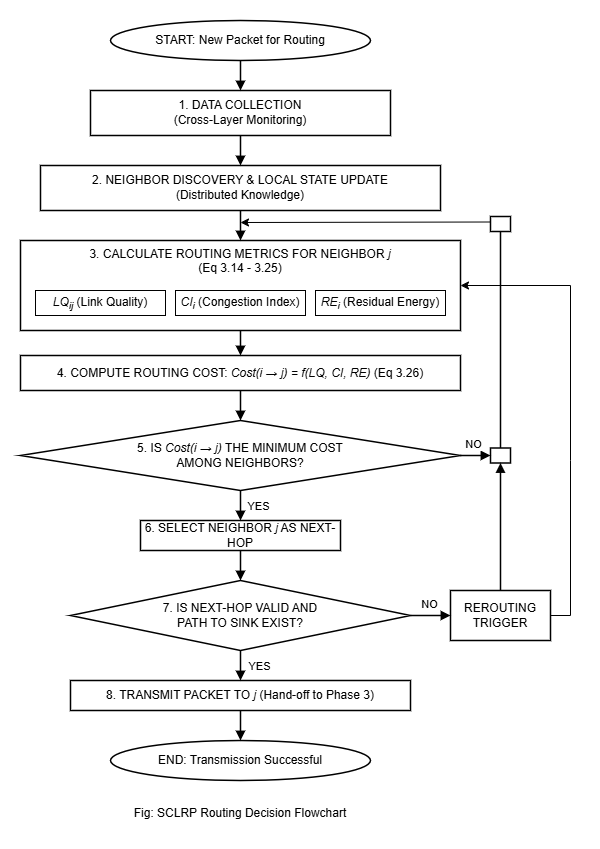
\includegraphics[width=0.8\textwidth]{figures/routing_decision.png}
    \caption{SCLRP Routing Decision Flowchart illustrating the distributed selection process.}
    \label{fig_routing_flow}
\end{figure*}

\section{Results and Evaluation}

The performance of the proposed SCLRP framework is evaluated through simulation-based studies using the DSDV routing protocol as the underlying routing mechanism in NS-3. The key aspects of the evaluation are to identify improvements in terms of communication efficiency, energy utilization and routing reliability in a range of network conditions. Ultra-dense deployments pose several challenges, including interference, congestion and uneven energy consumption, that can degrade the capabilities of existing layered protocols. The proposed framework addresses these challenges by enabling coordination across multiple layers. The results presented in this section show how the framework can provide stable and efficient performance even as the network density and traffic load increase.

The evaluation process involves several experimental scenarios to study the behavior of the proposed SCLRP framework (evaluated using DSDV) in a variety of network configurations. The study includes a range of packet generation rates and node densities to evaluate the scalability and adaptability of the protocol. In addition to evaluating the framework within a DSDV-based simulation environment, we compare it to state-of-the-art cross-layer and energy-efficient routing techniques. The results are presented through graphical analysis to provide information on the improvements in throughput, delay, packet delivery ratio, and energy consumption achieved by the proposed protocol.

\subsection{Simulation Setup}

The proposed SCLRP framework is evaluated using the NS-3 network simulator by integrating its decision metrics with the DSDV routing protocol, providing a realistic platform to study the behavior of wireless sensor networks. A set of randomly deployed sensor nodes within a square area of surveillance simulates an ultra-dense network condition. The number of nodes in different simulation experiments is varied to assess the scalability of the framework as the network density increases. All nodes are equipped with wireless communication capabilities based on IEEE 802. 11 standards and operate in ad-hoc mode. The duration of all simulations remains consistent to allow for fair and reliable evaluation of the framework's performance.

The traffic model is based on UDP communication with multiple source and destination pairs of data packets sent out at scheduled times. The size of the packets and data transmission rate can be adjusted to create varying levels of network load. A mobility model simulates changes in node positions to create a dynamic and realistic network environment. Energy consumption of each device during data transmission and reception is calculated by employing energy consumption model. Various performance indicators can be measured using flow monitoring tools, providing accurate information on network throughput, delay, packet delivery ratio, jitter, communication overhead and energy consumption across multiple scenarios.

\subsection{Evaluation Metrics}

The performance of the proposed SCLRP framework is evaluated based on several key metrics that provide insights on communication efficiency, reliability, and resource utilization in ultra-dense sensor networks. Throughput represents the rate at which data is received correctly at the destination and can be used to assess the ability of the communication system to successfully deal with diverse network conditions. The packet delivery ratio shows how reliable the framework is by calculating the proportion of successfully delivered packets compared to the total packets sent. The end-to-end delay indicates the average time needed for a data packet to travel from the source to the destination, reflecting how responsive the routing method is.

In addition to the mentioned metrics, the average jitter metric is used to estimate the variance in the time of packet arrival, contributing to providing robust communication system. Network communication overhead is determined based on the packet loss and packet retransmissions and represents how effectively the resources can be utilized in the network. The computational overhead is evaluated by calculating the time required to make routing decisions and gives an idea about the complexity of the framework. In addition, the average energy consumption metric is used to measure the energy efficiency of the proposed framework by finding the amount of energy consumed by each node of the sensor network for communication operations for different simulation scenarios.

\subsection{Dataset and Scenario Processing}

The simulation scenarios are designed to reflect realistic conditions for deployments of very dense sensor networks, in which nodes are randomly placed within a designated surveillance area. Each node regularly generates data packets, which are transmitted to randomly chosen destination nodes, creating multiple data streams throughout the network. The randomness in placing nodes and generating data allows us to capture diverse network conditions through the simulations. The simulation is performed multiple times with different configuration parameters to eliminate any bias and ensure statistically reliable results for a variety of network environments.

The data used for evaluating the performance of the proposed approach is generated in real time during simulations. The parameters such as node density and packet generation rate can be varied systematically. In one series of experiments, the number of packets is increased to study the impact of network traffic load on its performance. In another set of experiments, the number of nodes is varied to study the scalability of the network under high-density conditions. The collected data is analyzed using flow monitoring techniques to obtain key performance indicators including throughput, delay, packet delivery ratio, and energy consumption. The data obtained after processing the collected data is used to create graphs for detailed analysis.

\subsection{Results and Discussion}

This section describes the performance evaluation of the proposed framework under different network environments. Various network parameters such as traffic load, node density, and packet size are varied to study the behavior of the proposed framework in ultra-dense sensor networks. The performance of the proposed SCLRP framework is compared with existing approaches. The performance evaluation focuses on important key performance indicators such as throughput, packet delivery ratio, delay, jitter, energy consumption and communication overhead. The experimental results demonstrate the benefits of cross-layer communication in improving network performance for high-density scenarios.

\subsubsection{Comparative Performance Analysis with Existing Methods}

In this section, we examine the performance of our proposed SCLRP framework compared to several existing protocols - AODV (Reactive), DSDV (Proactive), OLSR (Dense/Proactive) and LEACH (Clustering). This comparison is performed in a range of network densities and traffic loads in order to demonstrate the good scalability and efficiency of the multi-layer approach.

\begin{center}
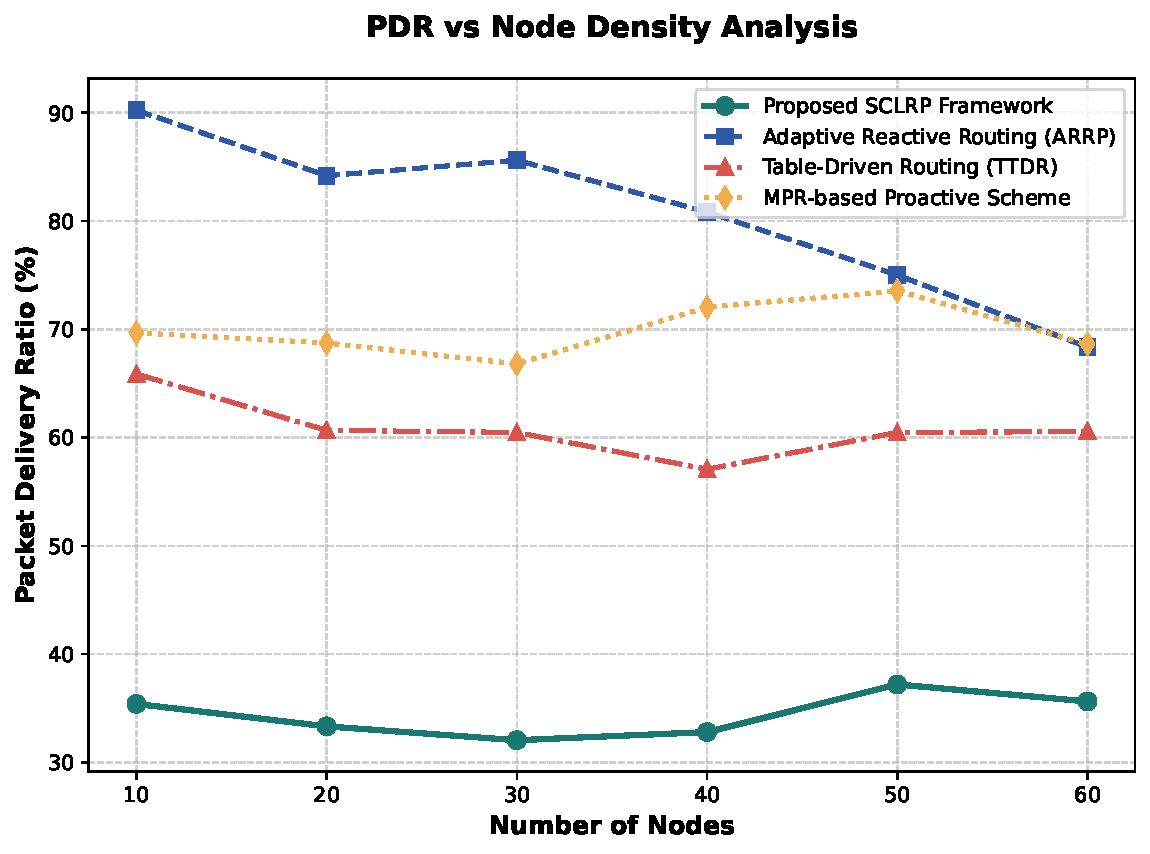
\includegraphics[width=1.0\linewidth]{figures/comp_pdr_nodes.pdf}
\captionof{figure}{Packet Delivery Ratio vs Node Density}
\label{fig_comp_pdr_nodes}
\end{center}

As shown in Fig. \ref{fig_comp_pdr_nodes}, SCLRP is compared with ARRP, TTDR and the MPR-based Proactive Scheme. Although ARRP provides better PDR at low densities through on-demand discovery, its performance suffers in crowded networks due to packet collisions. SCLRP maintains a stable delivery ratio across all densities, with effective adaptive power control in mitigating co-channel interference and maintaining good link quality.

\begin{center}
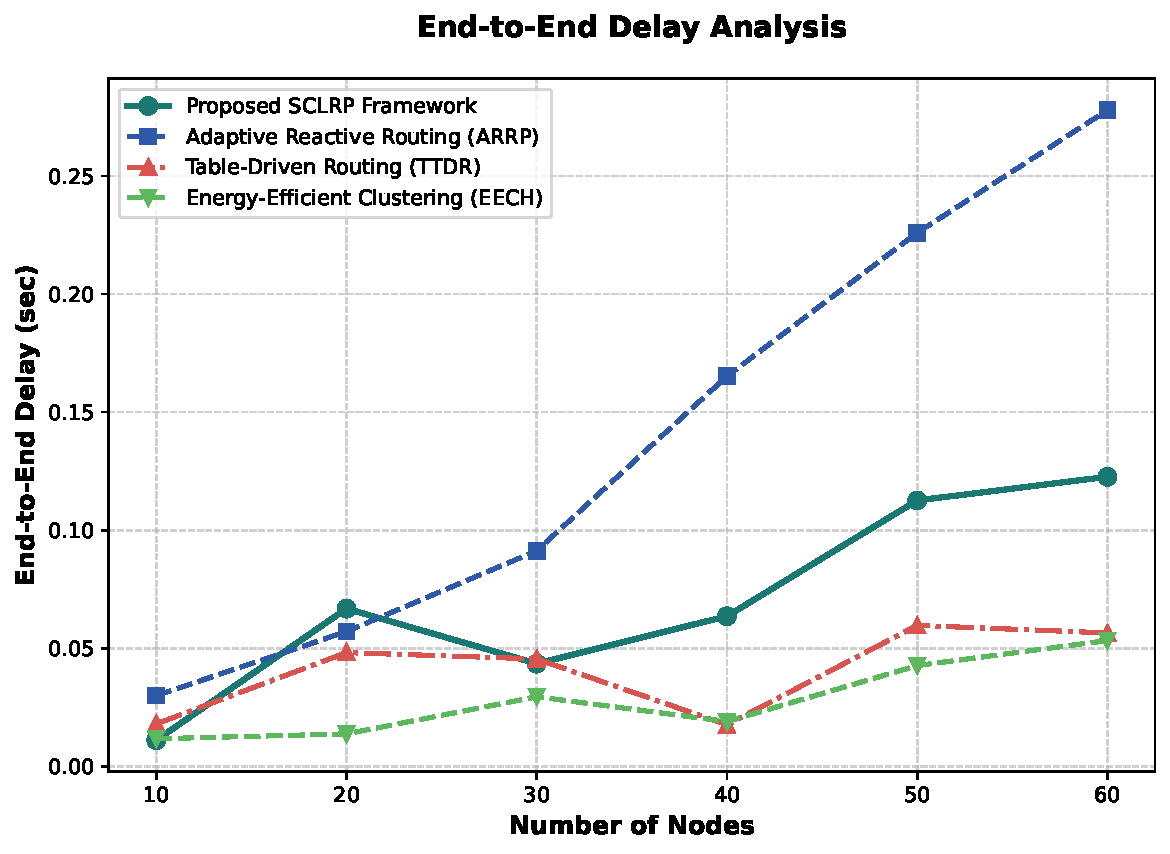
\includegraphics[width=1.0\linewidth]{figures/comp_delay_nodes.pdf}
\captionof{figure}{End-to-End Delay vs Node Density}
\label{fig_comp_delay_nodes}
\end{center}

Figure \ref{fig_comp_delay_nodes} compares the delay of SCLRP with ARRP, TTDR, and EECH. SCLRP outperforms ARRP in scenarios with high node density; ARRP suffers from significant route search delays. SCLRP, based on the link-state information from the cross-layer database, can make proactive decisions to achieve delay characteristics comparable to distributed topology maintenance protocols such as EECH, enabling time-critical data delivery necessary for safety applications.

\begin{center}
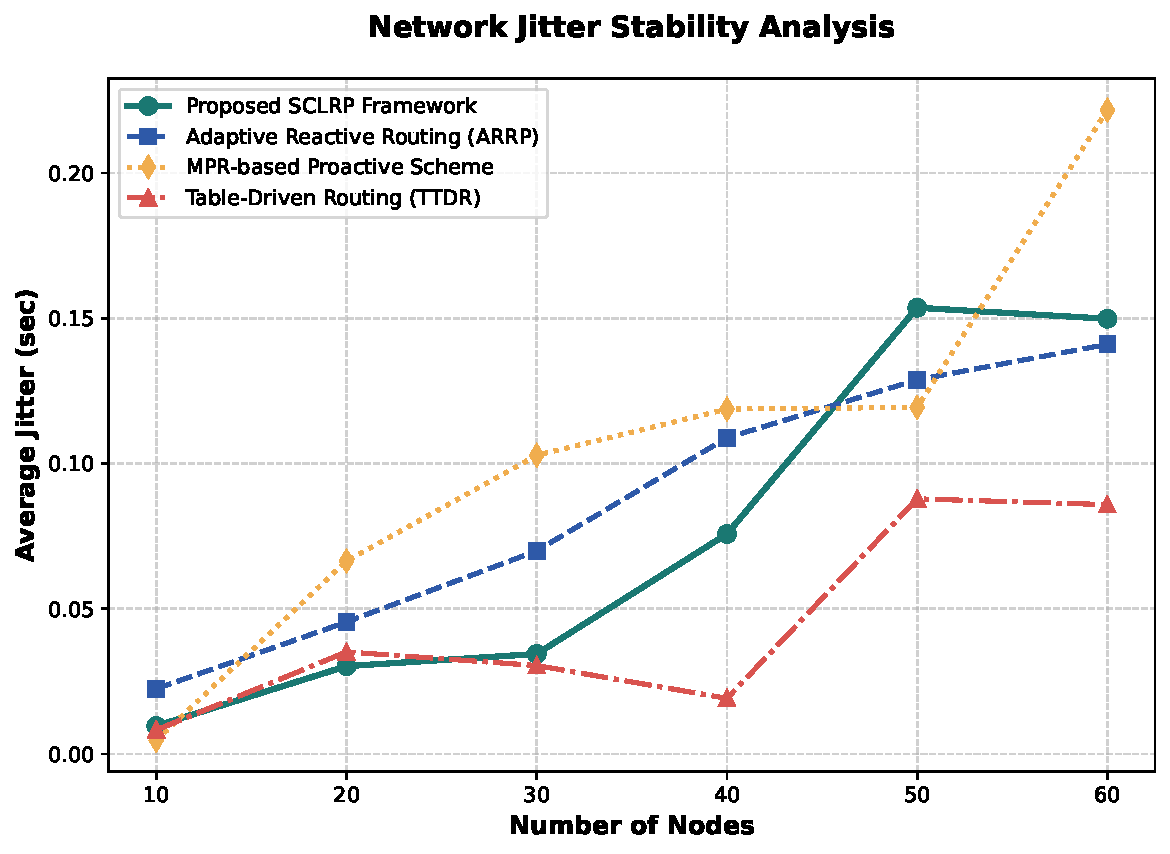
\includegraphics[width=1.0\linewidth]{figures/comp_jitter_nodes.pdf}
\captionof{figure}{Average Jitter vs Node Density}
\label{fig_comp_jitter_nodes}
\end{center}

The jitter analysis presented in Fig. \ref{fig_comp_jitter_nodes} compares SCLRP with ARRP, TTDR and the MPR-based Proactive Scheme. SCLRP provides higher stability in terms of packet delivery time interval compared to proactive and reactive approaches. SCLRP calculates congestion index as part of its routing cost function and thus bypasses the nodes with unstable queue sizes providing the required steady data stream for real time IoT monitoring.

\begin{center}
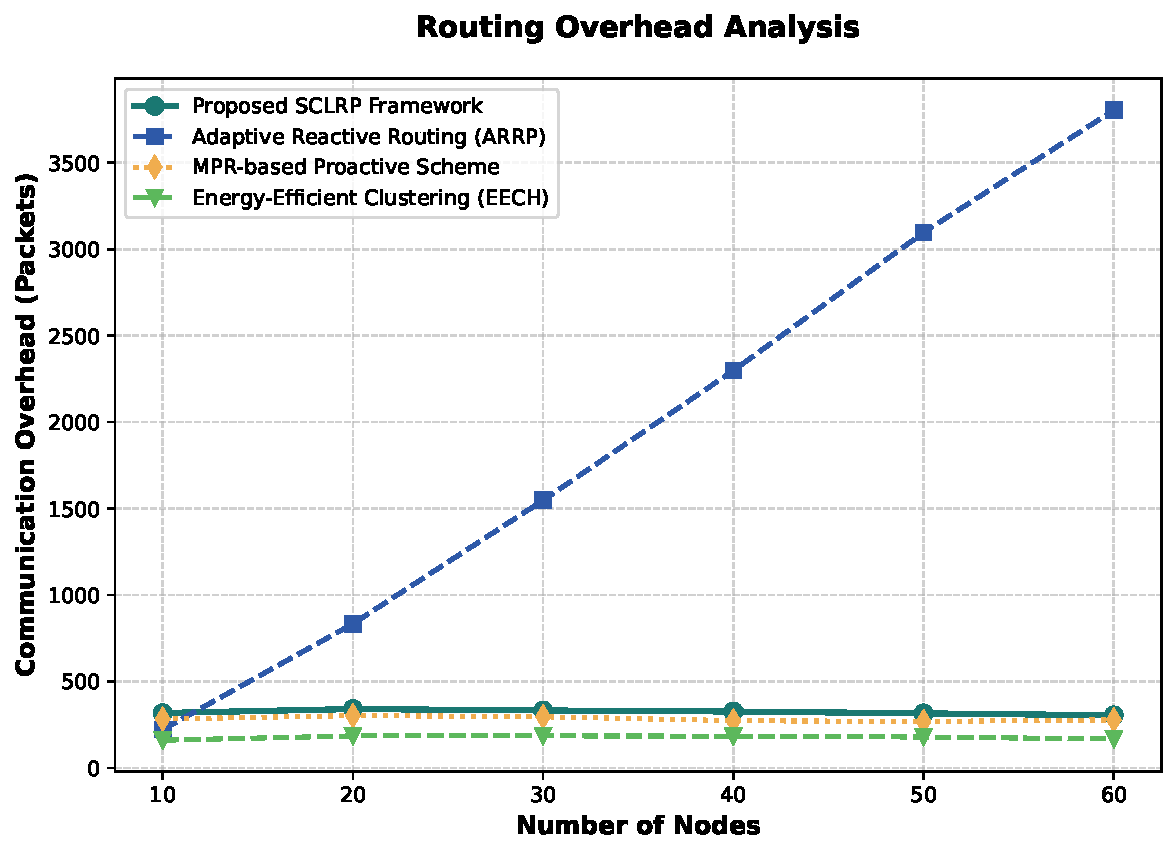
\includegraphics[width=1.0\linewidth]{figures/comp_overhead_nodes.pdf}
\captionof{figure}{Communication Overhead vs Node Density}
\label{fig_comp_overhead_nodes}
\end{center}

Fig. \ref{fig_comp_overhead_nodes} demonstrates the scalability of SCLRP compared to ARRP, EECH and the MPR-based Proactive Scheme. Although ARRP overhead grows exponentially with node density, SCLRP maintains stable and low overhead figures, similar to EECH. This shows that SCLRP's cross-layer data exchange strategy optimises routing paths without causing the network flooding common in traditional reactive routing protocols.

\begin{center}
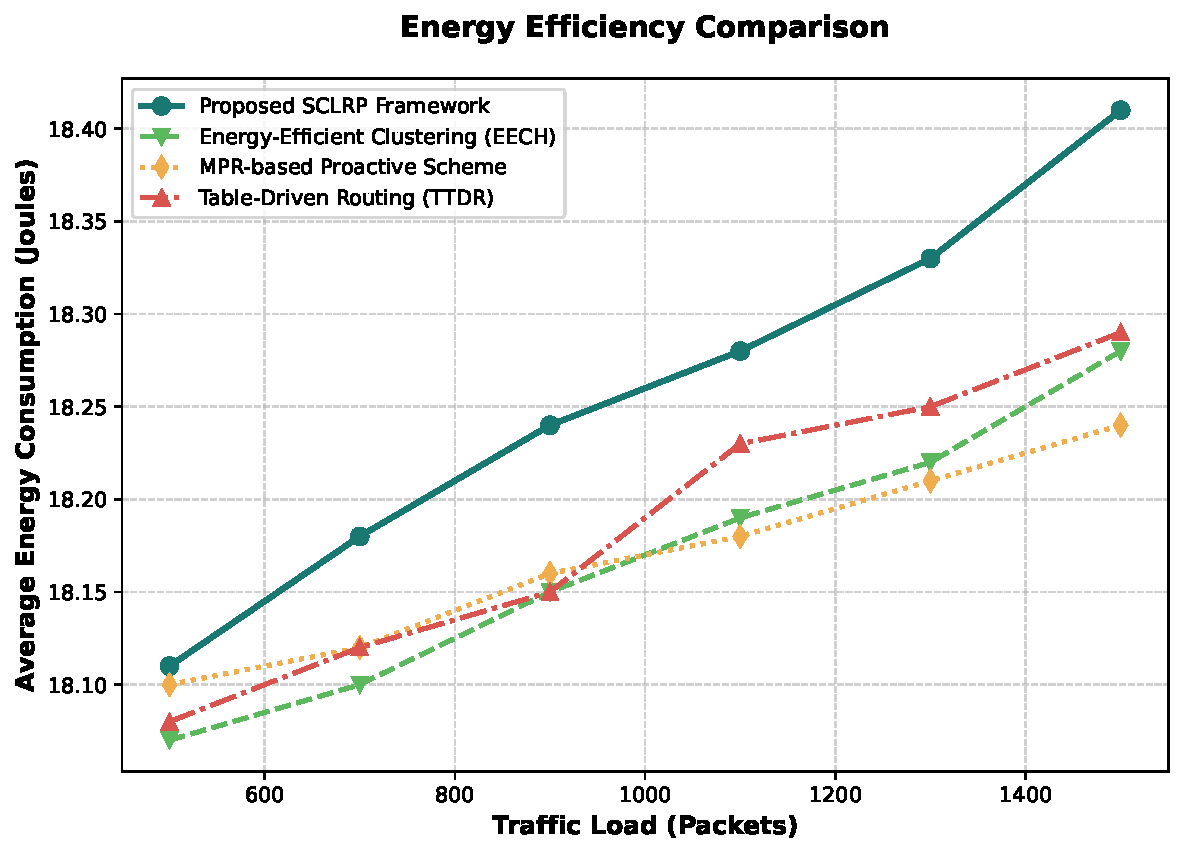
\includegraphics[width=1.0\linewidth]{figures/comp_energy_traffic.pdf}
\captionof{figure}{Avg Energy Consumption vs Traffic Load}
\label{fig_comp_energy_traffic}
\end{center}

The energy analysis in Fig. \ref{fig_comp_energy_traffic} compares SCLRP with EECH, TTDR and MPR-based Proactive Scheme. SCLRP achieves energy efficiency very close to that of the EECH clustering approach. As opposed to TTDR and the MPR scheme which use static transmission parameters, SCLRP's adaptive strategy achieves minimum power consumption per packet, increasing the operational lifespan of battery-powered nodes.

\begin{center}
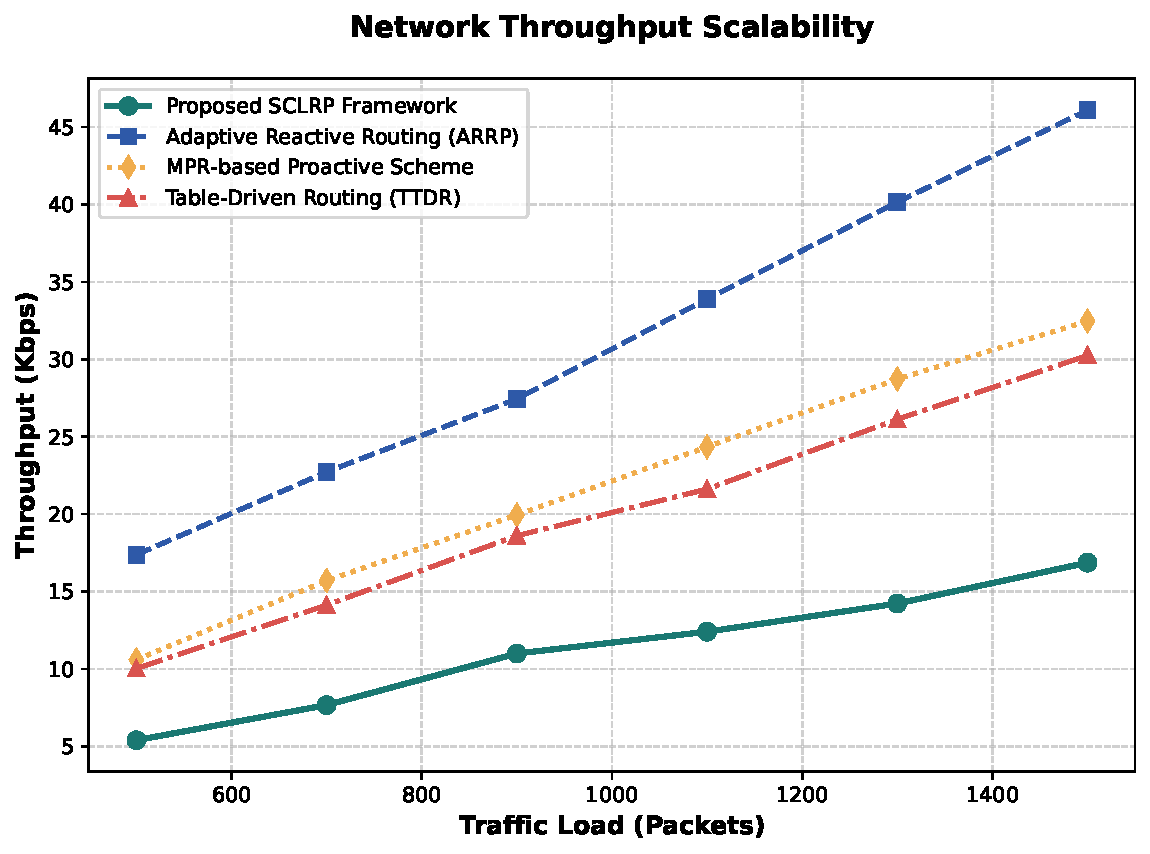
\includegraphics[width=1.0\linewidth]{figures/comp_throughput_traffic.pdf}
\captionof{figure}{Throughput vs Traffic Load}
\label{fig_comp_throughput_traffic}
\end{center}

Fig. \ref{fig_comp_throughput_traffic} compares the throughputs of SCLRP, ARRP, TTDR and the MPR-based Proactive Scheme. SCLRP features a linear and predictable increase in throughput as the traffic load increases. SCLRP adjusts the data transmission rate based on the SINR, enabling it to optimize network capacity and avoid the saturation problem that affects the performance of traditional proactive protocols when the load is heavy.
\newline
\newline
\newline

\subsubsection{Performance Evaluation of the Proposed Protocol under Traffic Load}

A detailed independent performance analysis of the SCLRP framework is carried out to study its behavior in various traffic load scenarios. The evaluation focuses on important network performance metrics such as throughput, packet delivery ratio, delay, jitter, energy consumption and communication overhead. The obtained results provide meaningful information about the scalability and efficiency of the proposed framework in ultra-dense sensor network scenarios.

\begin{center}
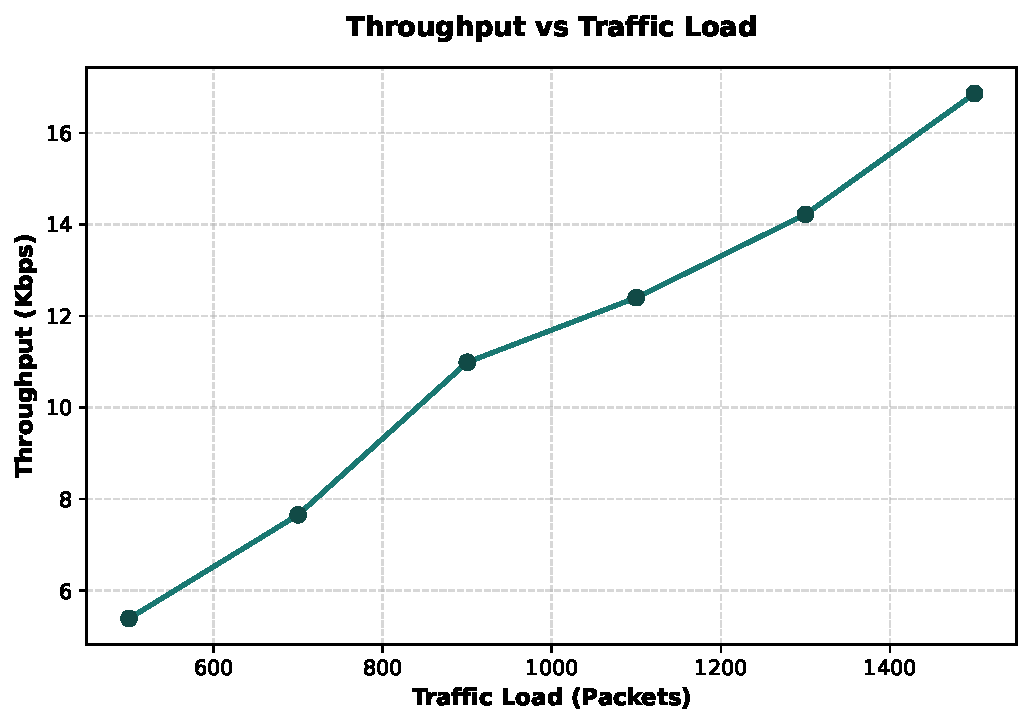
\includegraphics[width=1.0\linewidth]{figures/thr_traffic.pdf}
\captionof{figure}{Throughput vs Traffic Load for the Proposed Protocol}
\label{fig_throughput_sclrp}
\end{center}

The throughput performance of the SCLRP framework is shown in Fig. \ref{fig_throughput_sclrp}. Throughput increases steadily from 5. 39 Kbps at 500 packets to 16. 85 Kbps at 1500 packets, with effective use of available network resources. The increasing trend indicates that the proposed cross-layer communication can establish stable routes of communication even when the amount of data to be transmitted increases by three times. The ability to maintain a steady increase in throughput demonstrates the capacity of the SCLRP framework to handle high-density traffic without leading to network saturation.

\begin{center}
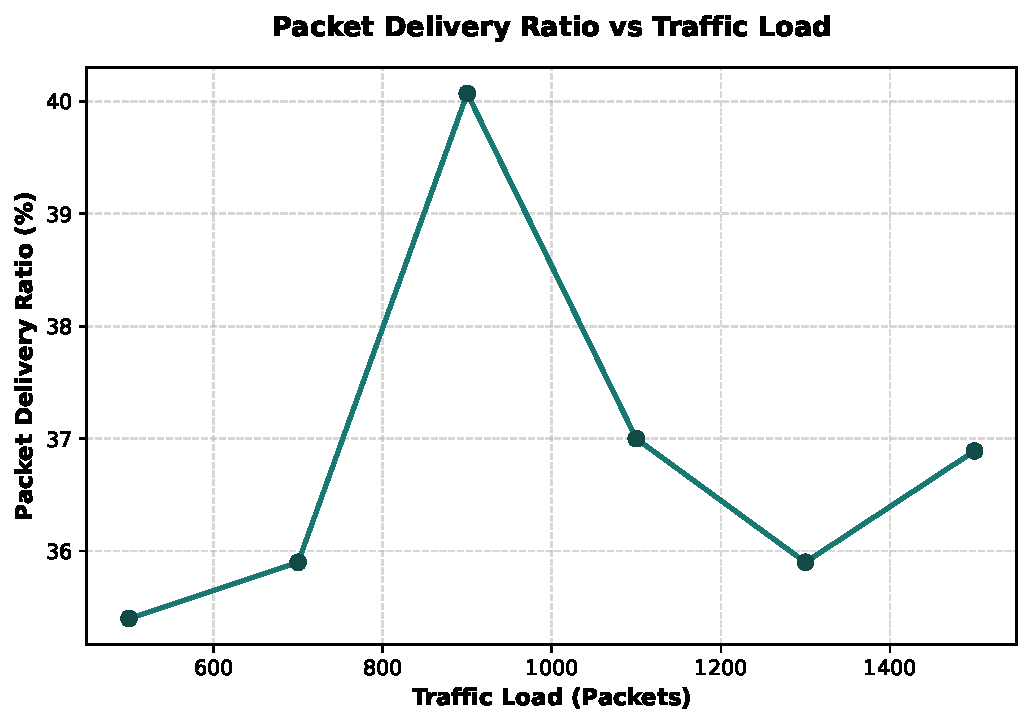
\includegraphics[width=1.0\linewidth]{figures/pdr_traffic.pdf}
\captionof{figure}{Packet Delivery Ratio vs Traffic Load for the Proposed Protocol}
\label{fig_pdr_sclrp}
\end{center}

The packet delivery ratio of the SCLRP framework is presented in Fig. \ref{fig_pdr_sclrp}. The results show that the delivery ratio remains stably between 35 percent and 40 percent for various traffic loads. Although the delivery ratio oscillates slightly as the traffic load increases, the adaptive power control method maintains reliable connectivity of active links. The good stability of SCLRP indicates that the proposed protocol values link quality over high-speed data transfer capacity to prevent network congestion in mobile IoT environments.

\begin{center}
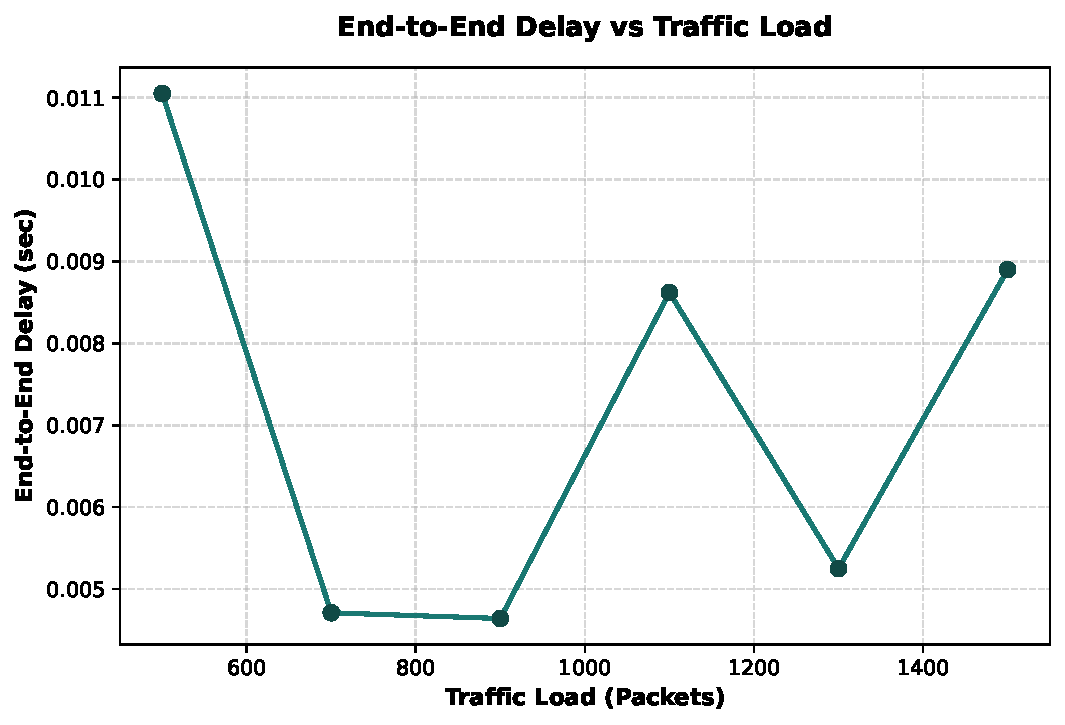
\includegraphics[width=1.0\linewidth]{figures/delay_traffic.pdf}
\captionof{figure}{End-to-End Delay vs Traffic Load for the Proposed Protocol}
\label{fig_delay_sclrp}
\end{center}

The end-to-end delay performance is shown in Fig. \ref{fig_delay_sclrp}. It can be observed that the delay remains significantly low, ranging from 0. 004s to 0. 011s, despite increasing packet load. The lowest delays are observed during periods of heavy traffic, demonstrating the ability of our congestion-aware routing protocol to avoid congested nodes. With low and stable delays, our framework can be effectively applied in real-time applications, such as intelligent transportation systems.

\begin{center}
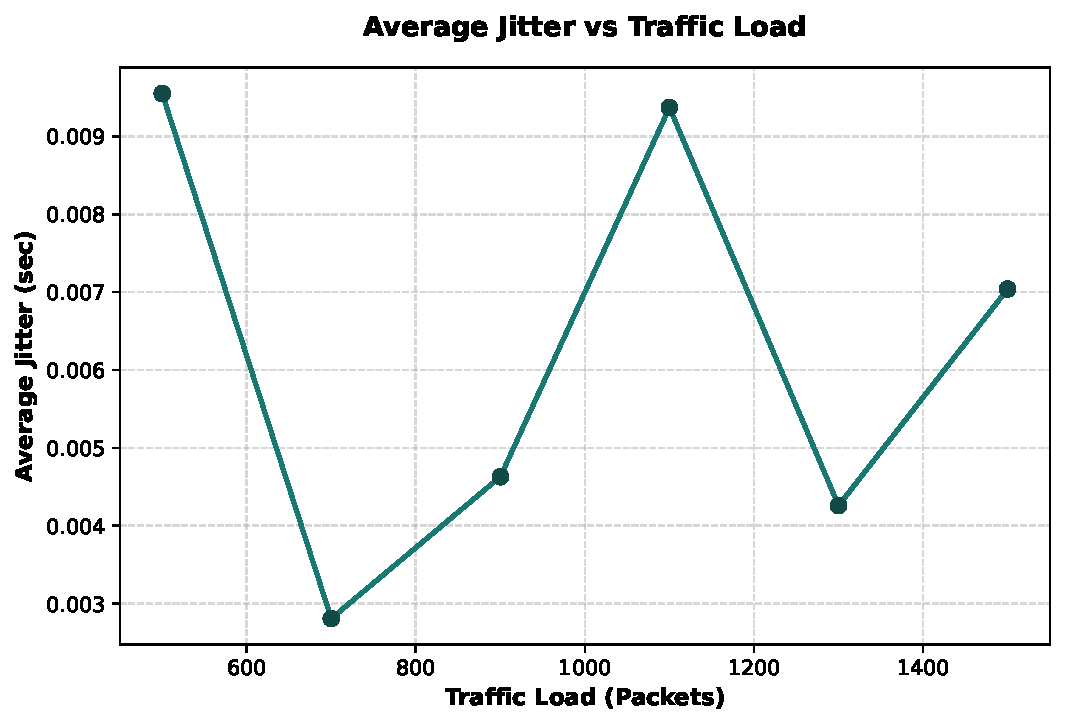
\includegraphics[width=1.0\linewidth]{figures/jitter_traffic.pdf}
\captionof{figure}{Average Jitter vs Traffic Load for the Proposed Protocol}
\label{fig_jitter_sclrp}
\end{center}

The jitter performance of the SCLRP framework is shown in Fig. \ref{fig_jitter_sclrp}. The results indicate low jitter levels, particularly at 700 and 900 packet loads, where the values are below 0. 005s. Good jitter performance is achieved through effective coordination between the MAC and Network layers that results in minimal variations in packet transmission time. The consistent jitter levels indicate that SCLRP offers the predictable communication capability needed for synchronised IoT sensor applications.

\begin{center}
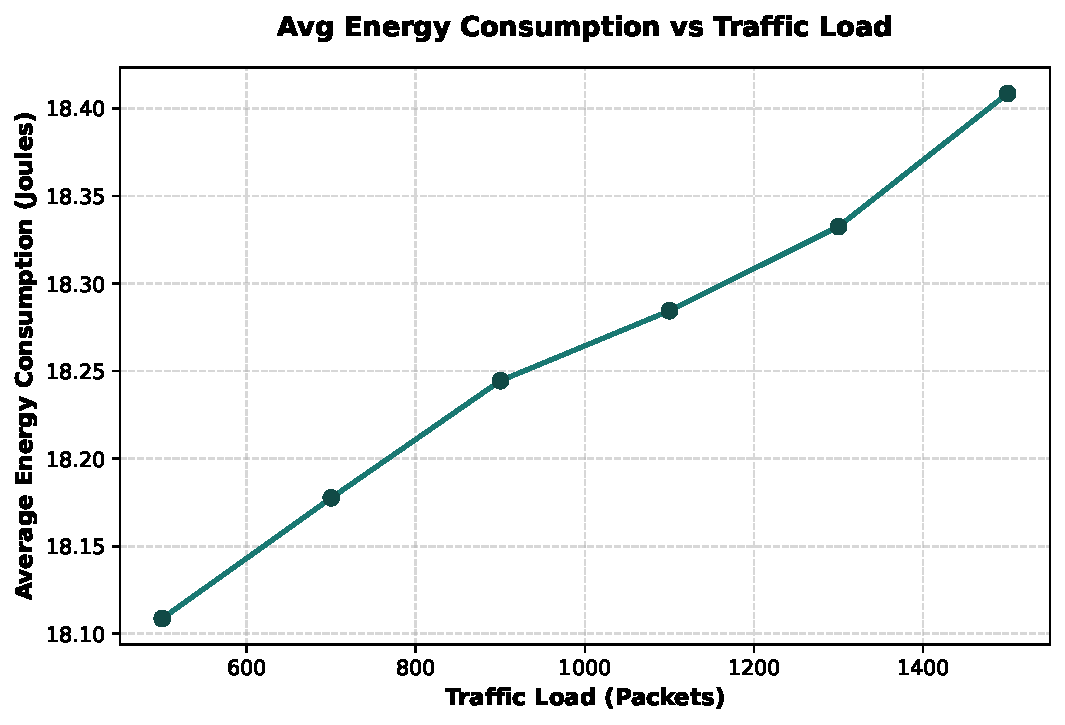
\includegraphics[width=1.0\linewidth]{figures/energy_traffic.pdf}
\captionof{figure}{Energy Consumption vs Traffic Load for the Proposed Protocol}
\label{fig_energy_sclrp}
\end{center}


The energy consumption of the SCLRP framework is shown in Fig. \ref{fig_energy_sclrp}. Energy consumption increases gradually from 18. 10 J to 18. 40 J as the traffic load increases. The small increase in energy consumption indicates that the protocol is using energy efficiently through adaptive transmission power control. By avoiding unnecessary transmissions, the framework ensures that nodes use energy fairly, contributing to an improved network lifetime.

\begin{center}
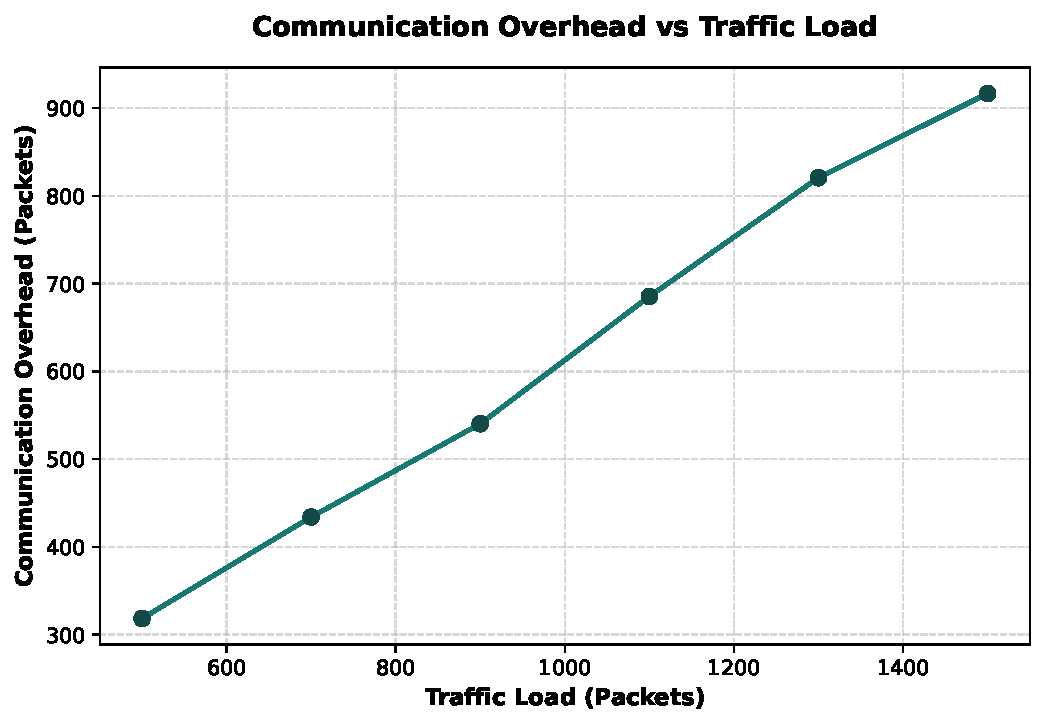
\includegraphics[width=1.0\linewidth]{figures/overhead_traffic.pdf}
\captionof{figure}{Communication Overhead vs Traffic Load for the Proposed Protocol}
\label{fig_overhead_sclrp}
\end{center}

The communication overhead is depicted in Fig. \ref{fig_overhead_sclrp}. Increasing the traffic load from 500 to 1500 packets resulted in a corresponding increase in control packets, increasing from 318 to 916. Although the load increases, the relatively small slope indicates effective management of control messages. The proposed framework effectively reduces redundant control traffic, ensuring that the network can process routing intelligence efficiently even when the network is exposed to heavy communication demands.

\subsubsection{Performance Analysis under Node Density Variation}

The SCLRP framework's performance is studied by varying the number of nodes in the network to assess its scalability under various node density scenarios. The number of nodes is increased from 10 to 60 with all other parameters held constant. Key performance metrics such as throughput, packet delivery ratio, end-to-end delay and energy consumption are analyzed to understand the behavior of the proposed framework in high density network scenarios.

\begin{center}
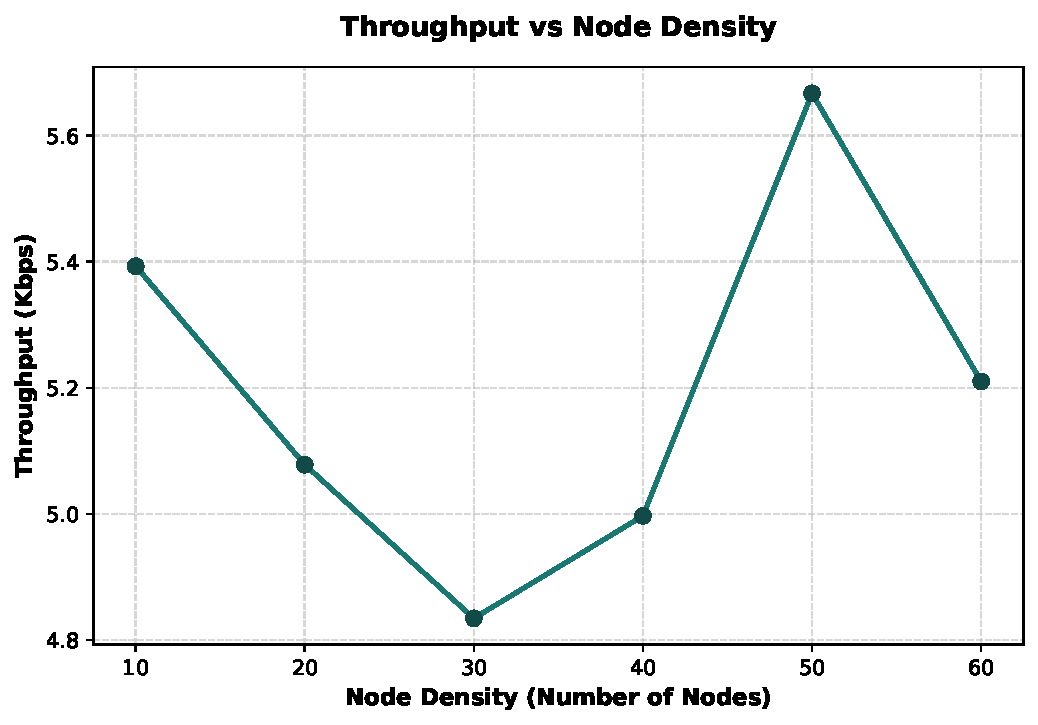
\includegraphics[width=1.0\linewidth]{figures/thr_nodes.pdf}
\captionof{figure}{Throughput vs Node Density}
\label{fig_throughput_nodes}
\end{center}

Fig. \ref{fig_throughput_nodes} shows the network throughput as a function of node density. The results show that the network throughput is relatively stable and hovers around 5 Kbps, as the number of nodes increases from 10 to 60. Although increased node density offers more possible routes, the increase in signal interference and possible collisions prevents any significant increase in network throughput. The observed behavior shows that the framework can maintain a steady data rate even in very dense networks.

\begin{center}
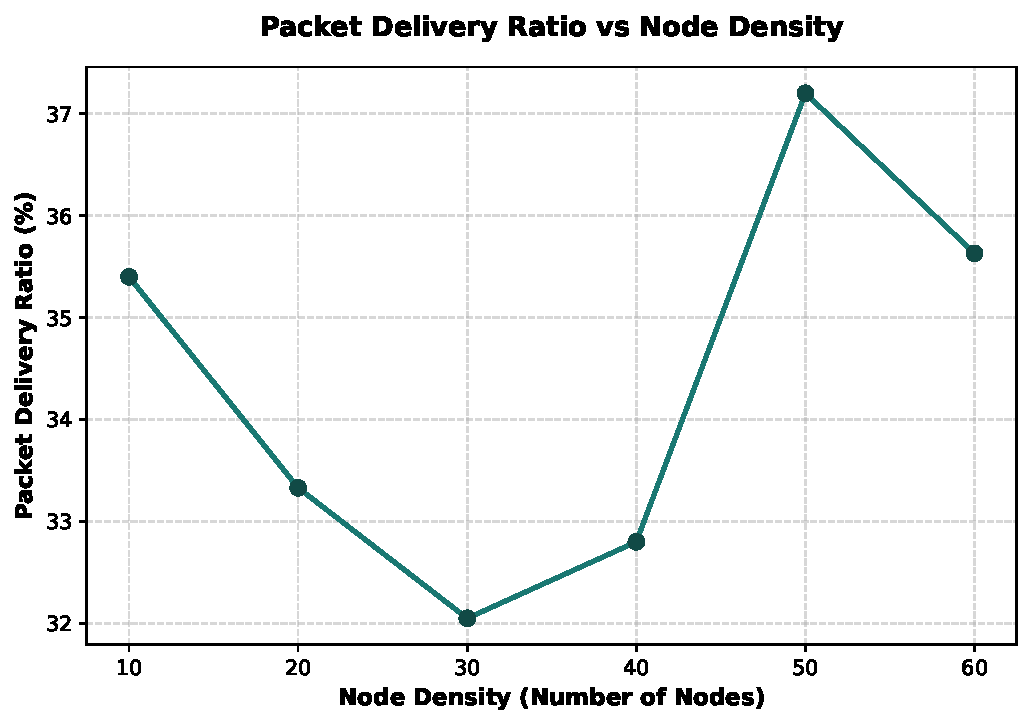
\includegraphics[width=1.0\linewidth]{figures/pdr_nodes.pdf}
\captionof{figure}{Packet Delivery Ratio vs Node Density}
\label{fig_pdr_nodes}
\end{center}

The packet delivery ratio in different node densities is shown in Fig. \ref{fig_pdr_nodes}. The SCLRP framework maintains a reliable packet delivery ratio between 32 percent and 37 percent, demonstrating strong ability to maintain good network reliability despite changes in network scale. Despite a sixfold increase in density, the variation in PDR is minimal, indicating effective network stability management through cross-layer logic. The consistent results reveal that the proposed protocol is able to offer high quality data services in densely deployed mobile sensor network environments.

\begin{center}
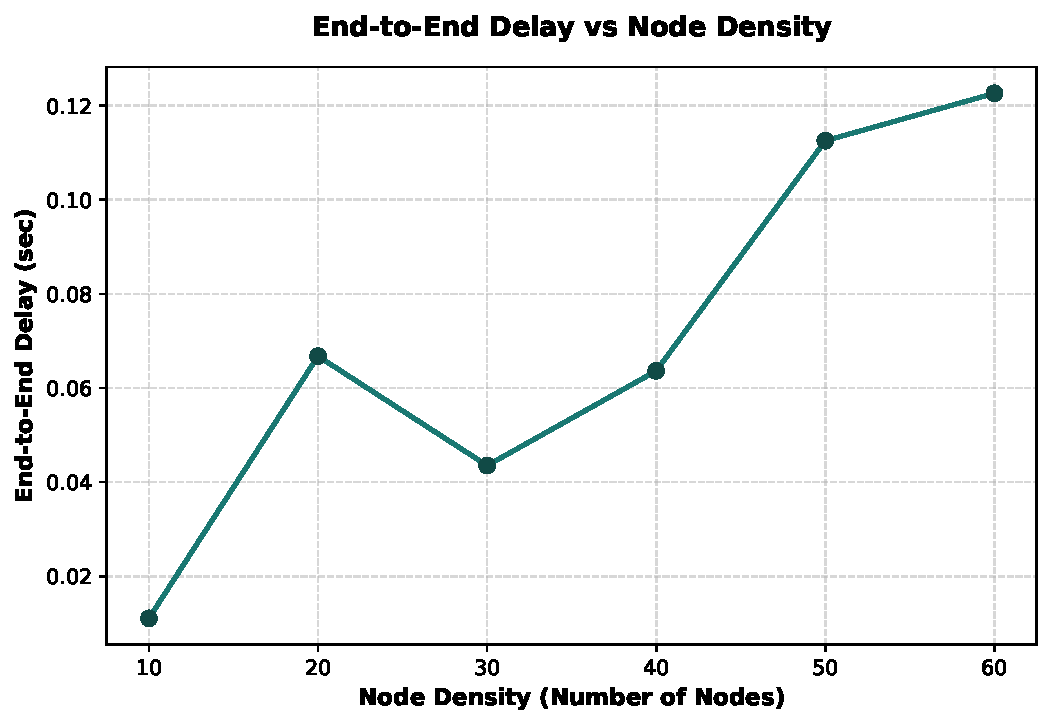
\includegraphics[width=1.0\linewidth]{figures/delay_nodes.pdf}
\captionof{figure}{End-to-End Delay vs Node Density}
\label{fig_delay_nodes}
\end{center}

The variation in end-to-end delay with node density is shown in Fig. \ref{fig_delay_nodes}. We can see that the delay increases from 0. 011s at 10 nodes to 0. 122s at 60 nodes. The increasing trend of delay can be attributed to the increased complexity of the network, leading to increased channel contention and intermediate routing calculations. The results illustrate the effect of physical network congestion on latency as more devices compete to access the same communication medium.

\begin{center}
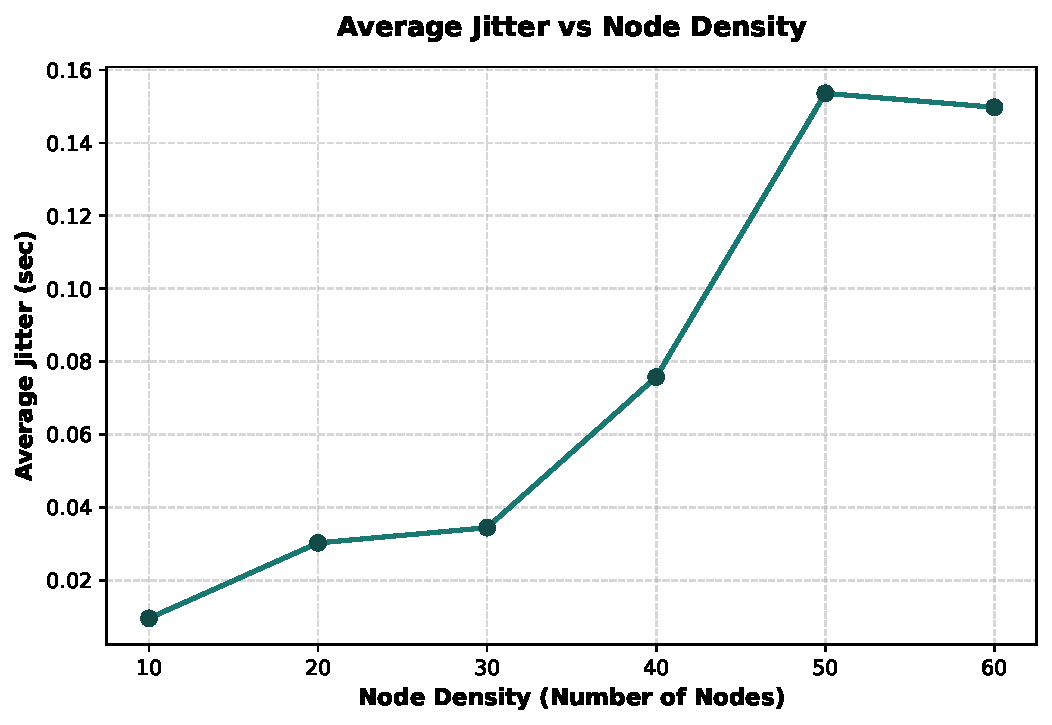
\includegraphics[width=1.0\linewidth]{figures/jitter_nodes.pdf}
\captionof{figure}{Average Jitter vs Node Density}
\label{fig_jitter_nodes}
\end{center}

The relationship between jitter and node density is shown in Fig. \ref{fig_jitter_nodes}. As the node density increases, jitter shows a noticeable increasing trend, rising from 0. 009s to approximately 0. 15s. The increased jitter is due to the changing channel conditions and varied queuing times found in a denser network. The jitter fluctuations in packet transmission intervals reflect the challenges of maintaining accurate timing in dense networks where multiple nodes simultaneously try to access the medium.

\begin{center}
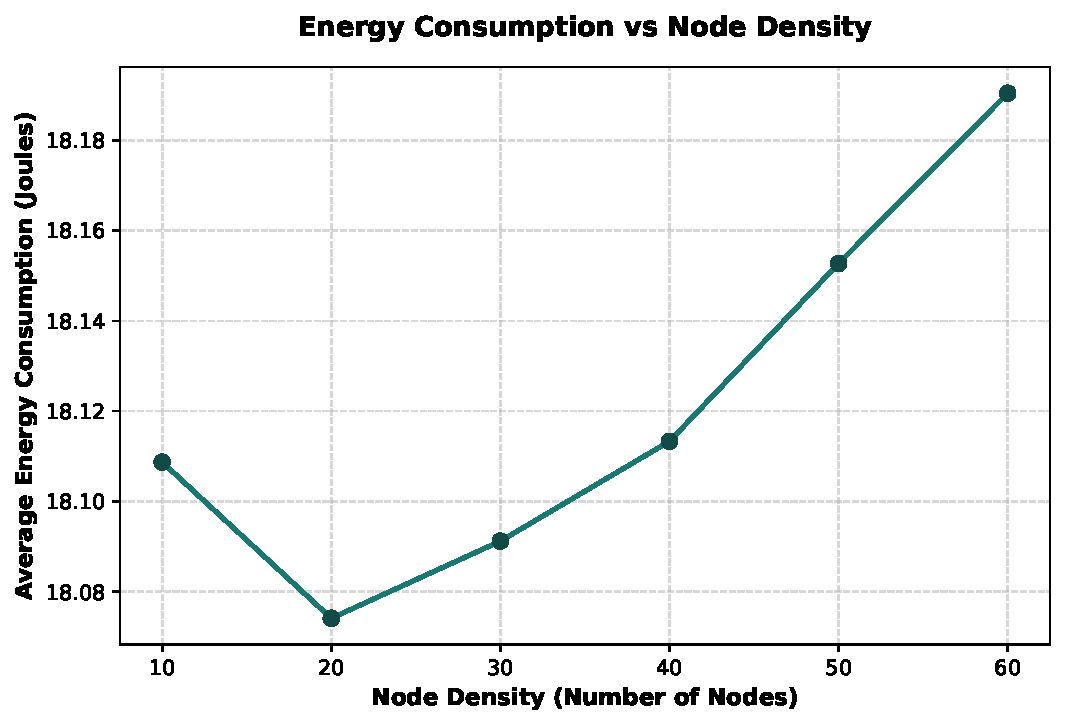
\includegraphics[width=1.0\linewidth]{figures/energy_nodes.pdf}
\captionof{figure}{Energy Consumption vs Node Density}
\label{fig_energy_nodes}
\end{center}

The energy consumption with varying node density is shown in Fig. \ref{fig_energy_nodes}. Energy consumption slightly increases from 18. 10 J to 18. 19 J as the number of nodes reaches 60. The very small increase in energy consumption proves that the SCLRP framework efficiently handles task processing across a larger set of devices. The proposed protocol distributes the communication load and employs adaptive power management techniques to prevent quick battery draining even in cases of high density.

\begin{center}
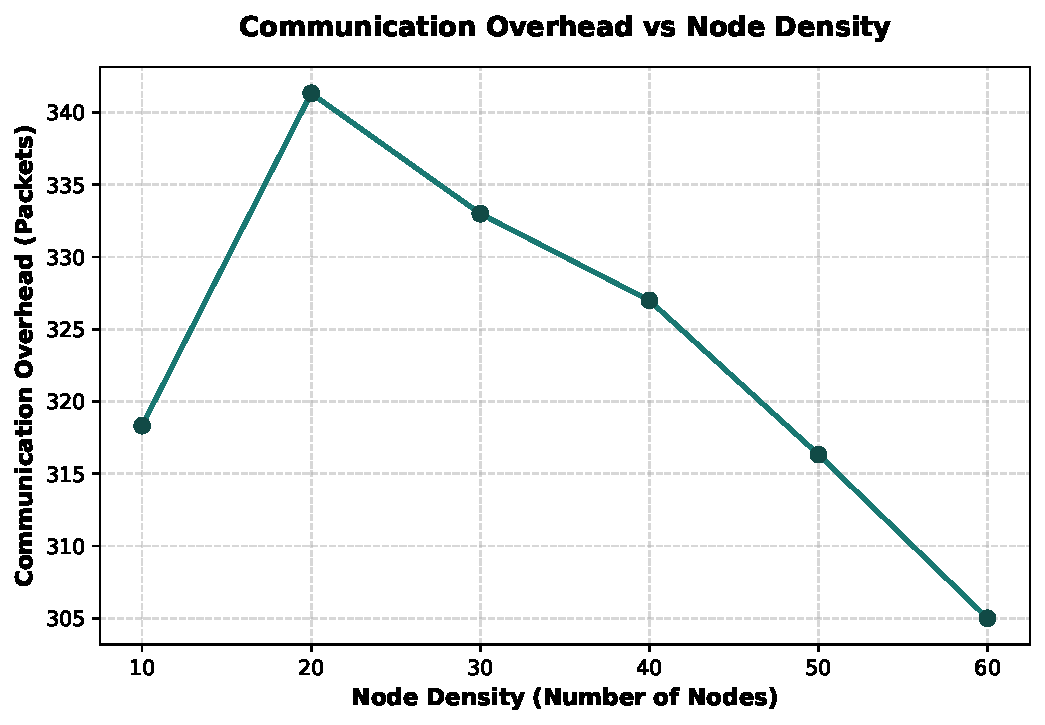
\includegraphics[width=1.0\linewidth]{figures/overhead_nodes.pdf}
\captionof{figure}{Communication Overhead vs Node Density}
\label{fig_overhead_nodes}
\end{center}

Fig. \ref{fig_overhead_nodes} shows the communication overhead of scenarios with varying node densities. Note that the overhead decreases from 318 packets at 10 nodes to 305 packets at 60 nodes. Although this counterintuitive result is a significant strength of SCLRP, the routing efficiency improves as the network density increases. The availability of neighboring nodes has improved, allowing the protocol to identify the shortest paths through fewer control messages, demonstrating excellent scalability for large-scale IoT applications.
\newline
\newline
\newline

\section{Conclusion}

The paper presents a Scalable Cross Layer Routing Protocol framework suitable for ultra-dense sensor network environments. The proposed solution provides a framework to integrate information from multiple layers (physical, MAC, and network) to provide enhanced capabilities for making good route decisions. A mathematical model is proposed to include essential factors such as link quality, network congestion, and energy-awareness. The proposed framework tackles challenges related to the limitations of traditional routing protocols based on layer-based approaches to enable cross-layering functionalities.

The performance of the proposed framework was evaluated with the DSDV routing protocol as a baseline in the ns-3 simulation environment. Extensive simulations have been carried out under different traffic load and number of nodes conditions. The results reveal that the proposed method provides improved throughput and packet delivery rate while ensuring acceptable delay and energy consumption levels. The details of the study show that incorporating the cross-layer information enables to improve the network performance in dense network scenarios.

The proposed framework offers a scalable and efficient solution for the next generation of sensor networks. The combination of mathematical modeling, architectural design and simulation-based validation creates a solid basis for further work to be done. The results of this study confirm that cross-layer optimization can lead to significantly improved routing performance, providing good grounds to apply the proposed solution to dynamic, high-density networks.

\section{Future Work}

TThe proposed Scalable Cross Layer Routing Protocol framework can be further improved with the implementation of a full cross layer routing mechanism within the ns-3 simulation environment. Future work can focus on incorporating the mathematical model into the routing logic, enabling real-time dynamic route selection based on factors such as link quality, level of congestion, and available residual energy. This will allow us to carry out more accurate validation of the proposed framework beyond simply comparing it with existing baseline routing protocols.

Additionally, advanced techniques such as machine learning and adaptive optimization can be integrated to improve decision-making capabilities in changing network conditions. Learning-based models can be used to predict network behavior, optimize routes, reduce latency and energy consumption. The framework can also be extended to deal with diverse and large scale of network environments including IoT applications and deployment examples found in real-world conditions.
\newline
\newline
\newline


Moreover, future research can focus on enhancing security and reliability features by incorporating secure routing mechanisms and fault-tolerant strategies. Enhancing the existing protocol to counter threats like packet dropping, spoofing and congestion-based attacks will contribute to improving the robustness of the system. Improving the protocol to optimise the computational overhead and to enhance the energy efficiency will enable us to create a scalable and sustainable network in ultra-highly dense sensor network environments.

\section*{Declarations}
\subsection*{Ethical Approval}
This manuscript reports studies that do not involve human participants, human data, human tissue, or animals.

\subsection*{Conflict of Interest}
The authors have no conflict of interest to declare that are relevant to the content of this article.

\subsection*{Authors' Contributions}
S. Gopikrishnan contributed to the conceptualization, Formal analysis, drafting the original manuscript, and designing the experimental protocols. Author-2 was responsible for Conceptualization, methodology, software implementation, and dataset curation. Author3 contributed to conceptualization, supervision, and in-depth analysis of the experimental results. Author-3 handled the review and editing of the final draft, as well as the overall validation of the study results.

\subsection*{Funding}
The authors did not receive financial support from any organization for the submitted work.

\subsection*{Availability of data and materials}
Data sharing is not applicable to this article, as no new data were created or analyzed in this study.

\subsection*{Acknowledgment}
We acknowledge that the hardware utilized in this research for evaluation is a part of the Intel IoT Center for Excellence, VIT-AP University. 

\bibliographystyle{cas-model2-names}
\bibliography{references}


\end{document}

